\documentclass[11pt]{article}
\usepackage[utf8]{inputenc}
\usepackage[T1]{fontenc}
\usepackage{amsmath,amssymb,graphicx,url,tabularx,booktabs}
\usepackage[margin=1in]{geometry}
\renewcommand{\thefigure}{S\arabic{figure}}
\title{Supplementary Material for ``Defect-Tolerant Design of Lead-Free RbGeI3 Solar Cells: From SCAPS-1D Optimization to Manufacturing Tolerances, Benchmarked Against CsGeI3''}
\author{Md.\ Abdul Malek Fahim and Hussain Touhid Siddiquee\thanks{Corresponding author: touhidsiddiqueeraj@gmail.com}}
\begin{document}
\maketitle

\section*{S1.\ One-at-a-time sweep details}
Full per-parameter traces for the eleven sequential optimization steps summarized in Section~V.B of the main text.
\subsection*{Effect of absorber layer thickness}
Thickness sets the trade-off between light capture and recombination: a thicker absorber absorbs more photons and lifts J$_{\mathrm{SC}}$, up to the point where the extra volume becomes a recombination liability.
PCE peaks at 0.7 $\mu$m (20.70\%) and eases off beyond it as recombination grows. J$_{\mathrm{SC}}$ climbs steadily with thickness, 28.14 to 34.11 mA/cm$^{2}$, while V$_{\mathrm{OC}}$ slides from 0.823 to 0.767 V. The 0.7 $\mu$m point, where the two effects balance, is the one we keep. The upper end of this J$_{\mathrm{SC}}$ range (34.11 mA/cm$^{2}$) exceeds the single-gap SQ limit at 1.4 eV ($\approx$33 mA/cm$^{2}$); it was recorded with the early Step-1 deck whose extended sub-gap absorption (cutoff toward $\approx$1.2 eV, SQ $\approx$40 mA/cm$^{2}$) accommodates it. Re-simulation of the thickness sweep with the consolidated uniform-1.4 eV deck gives J$_{\mathrm{SC}}$ 25.2--31.3 mA/cm$^{2}$ (all below SQ) with the same peak-plateau shape (plateau 0.7--1.0 $\mu$m within 0.06 points), so the 0.7 $\mu$m choice stands.


\begin{figure}[htbp]
\centering
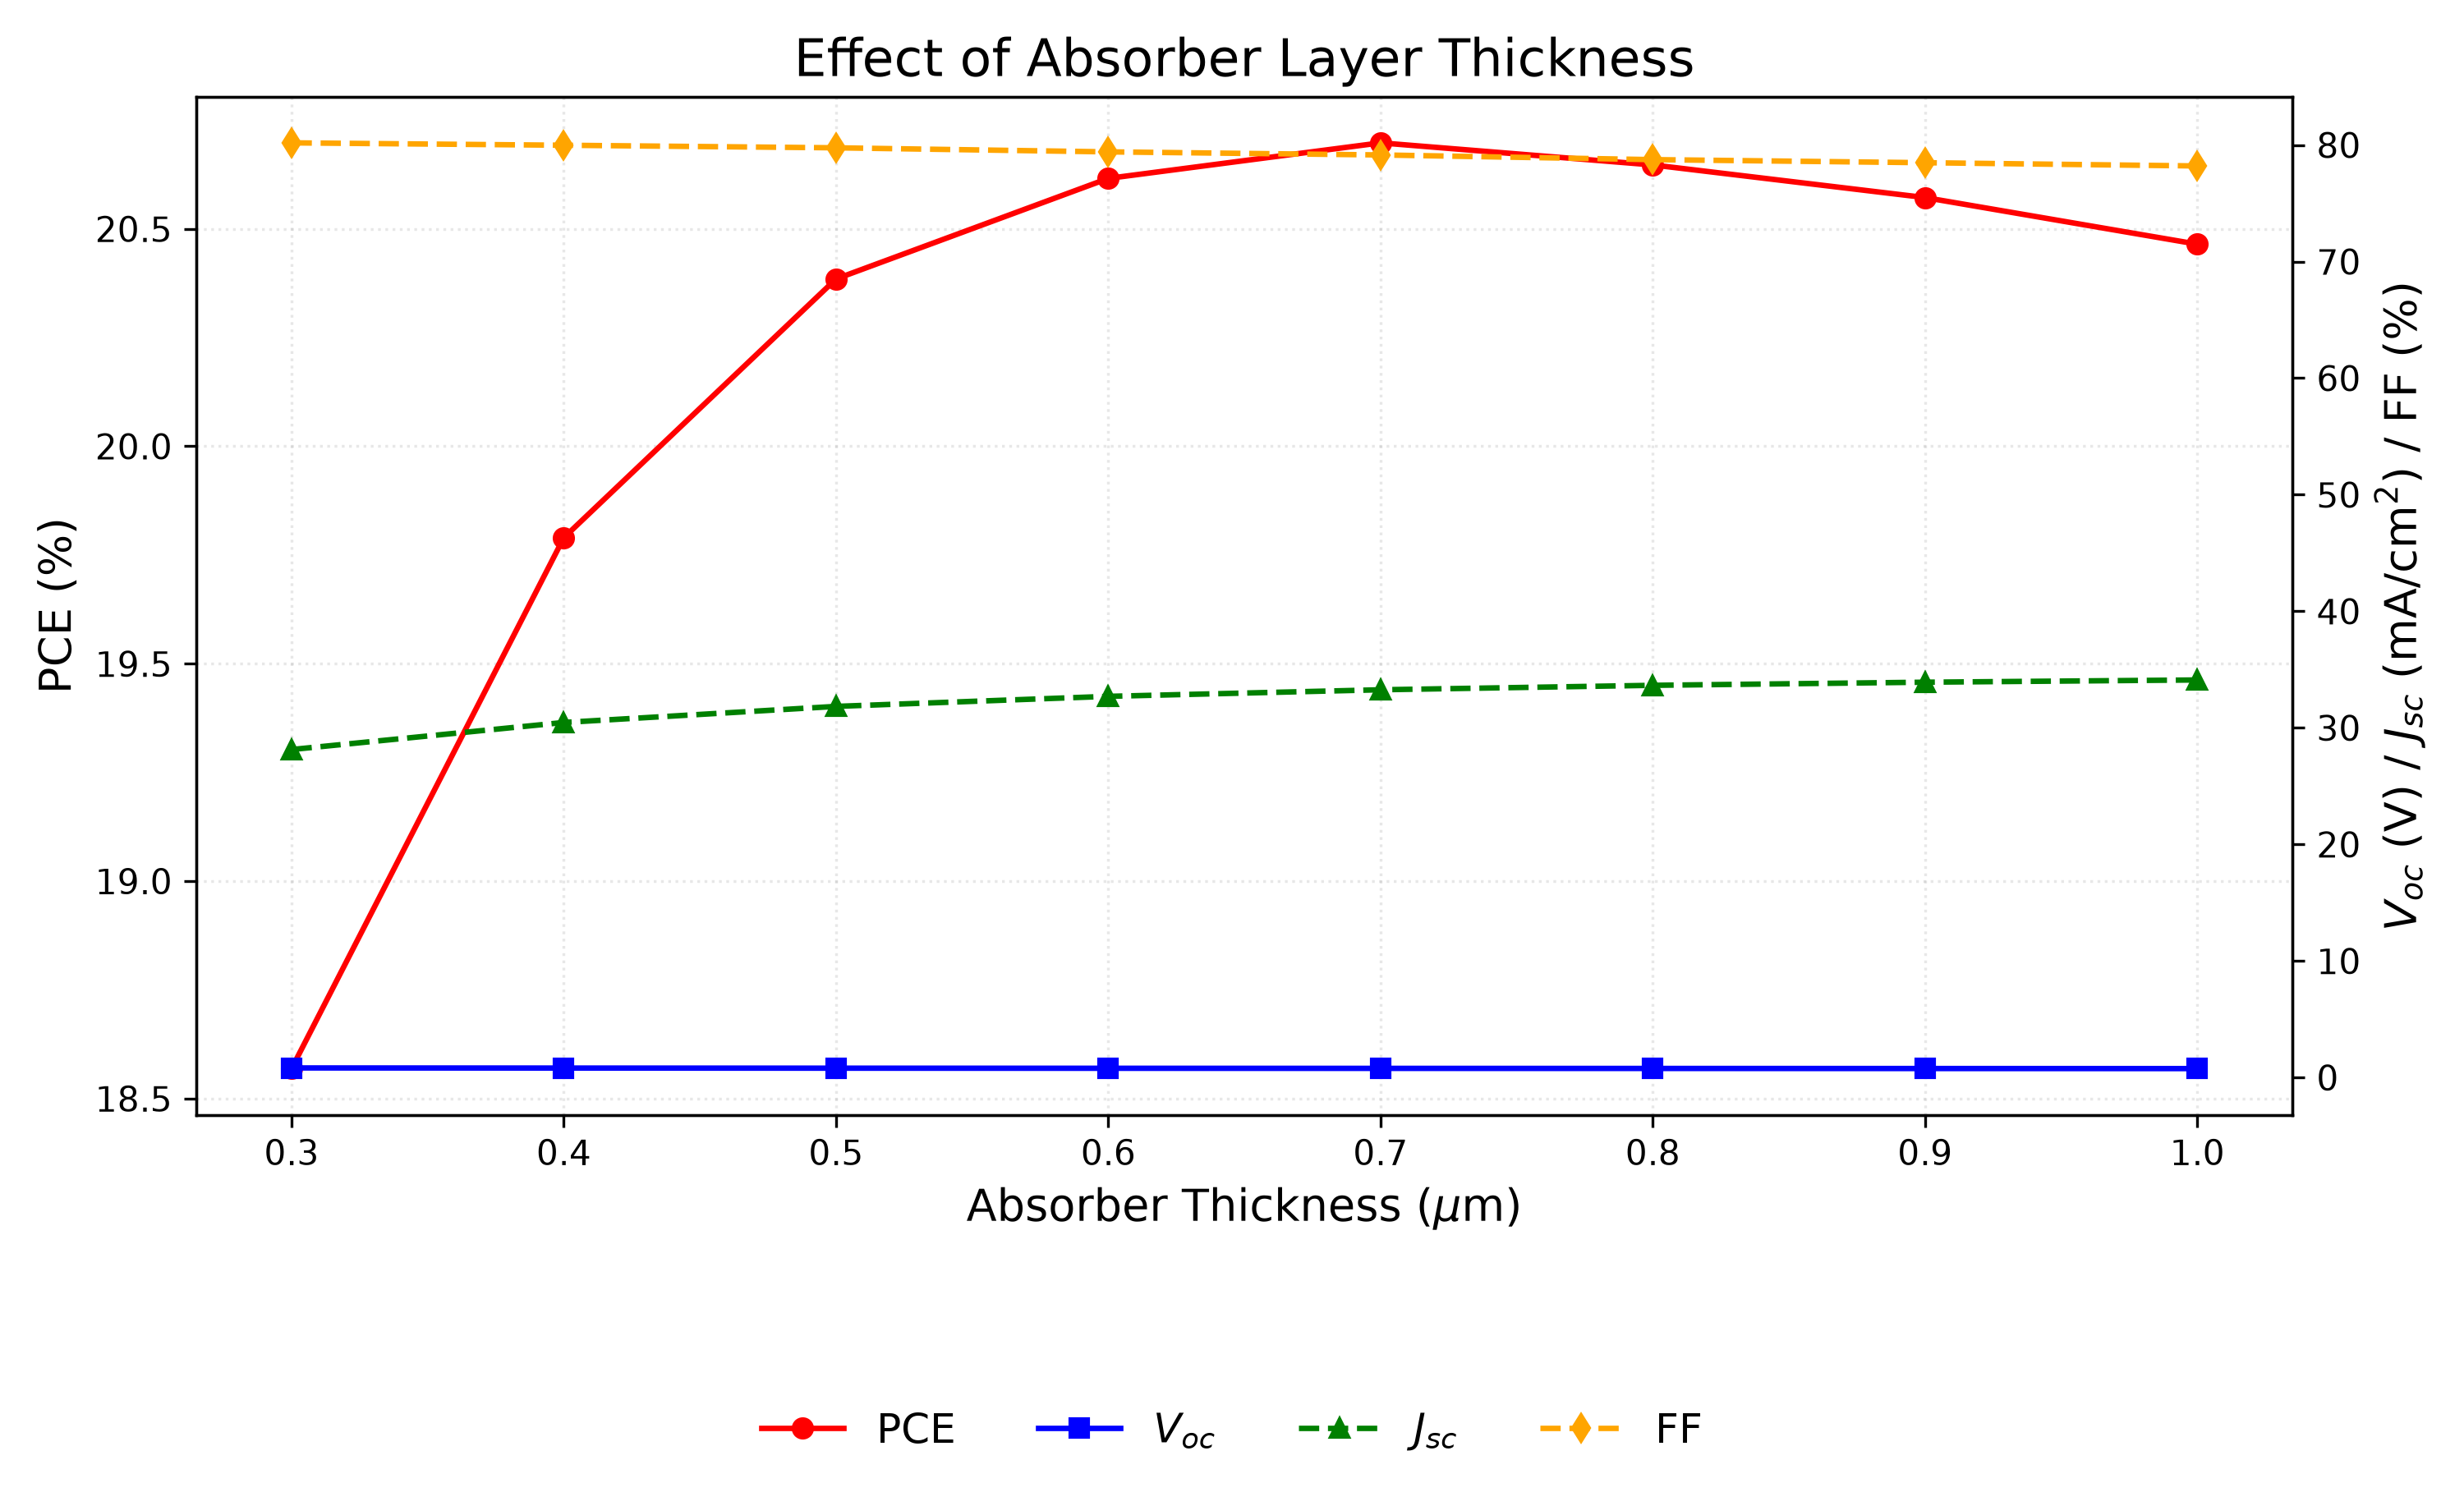
\includegraphics[width=0.85\linewidth]{figs/fig3.png}
\caption{Variation of PCE, V$_{\mathrm{OC}}$, J$_{\mathrm{SC}}$, and FF with RbGeI$_{3}$ absorber thickness. PCE peaks at 0.7 $\mu$m, beyond which recombination losses reduce efficiency.}
\end{figure}

\subsection*{Effect of absorber dielectric constant}
The dielectric constant barely matters. Raising $\epsilon$r from 15 to 23.1 moves PCE from 19.92\% to 19.79\%, a shift carried almost entirely by V$_{\mathrm{OC}}$ (0.819 to 0.812 V); J$_{\mathrm{SC}}$ and FF are essentially unchanged. With nothing to gain at the high end, we keep $\epsilon$r = 15.


\begin{figure}[htbp]
\centering
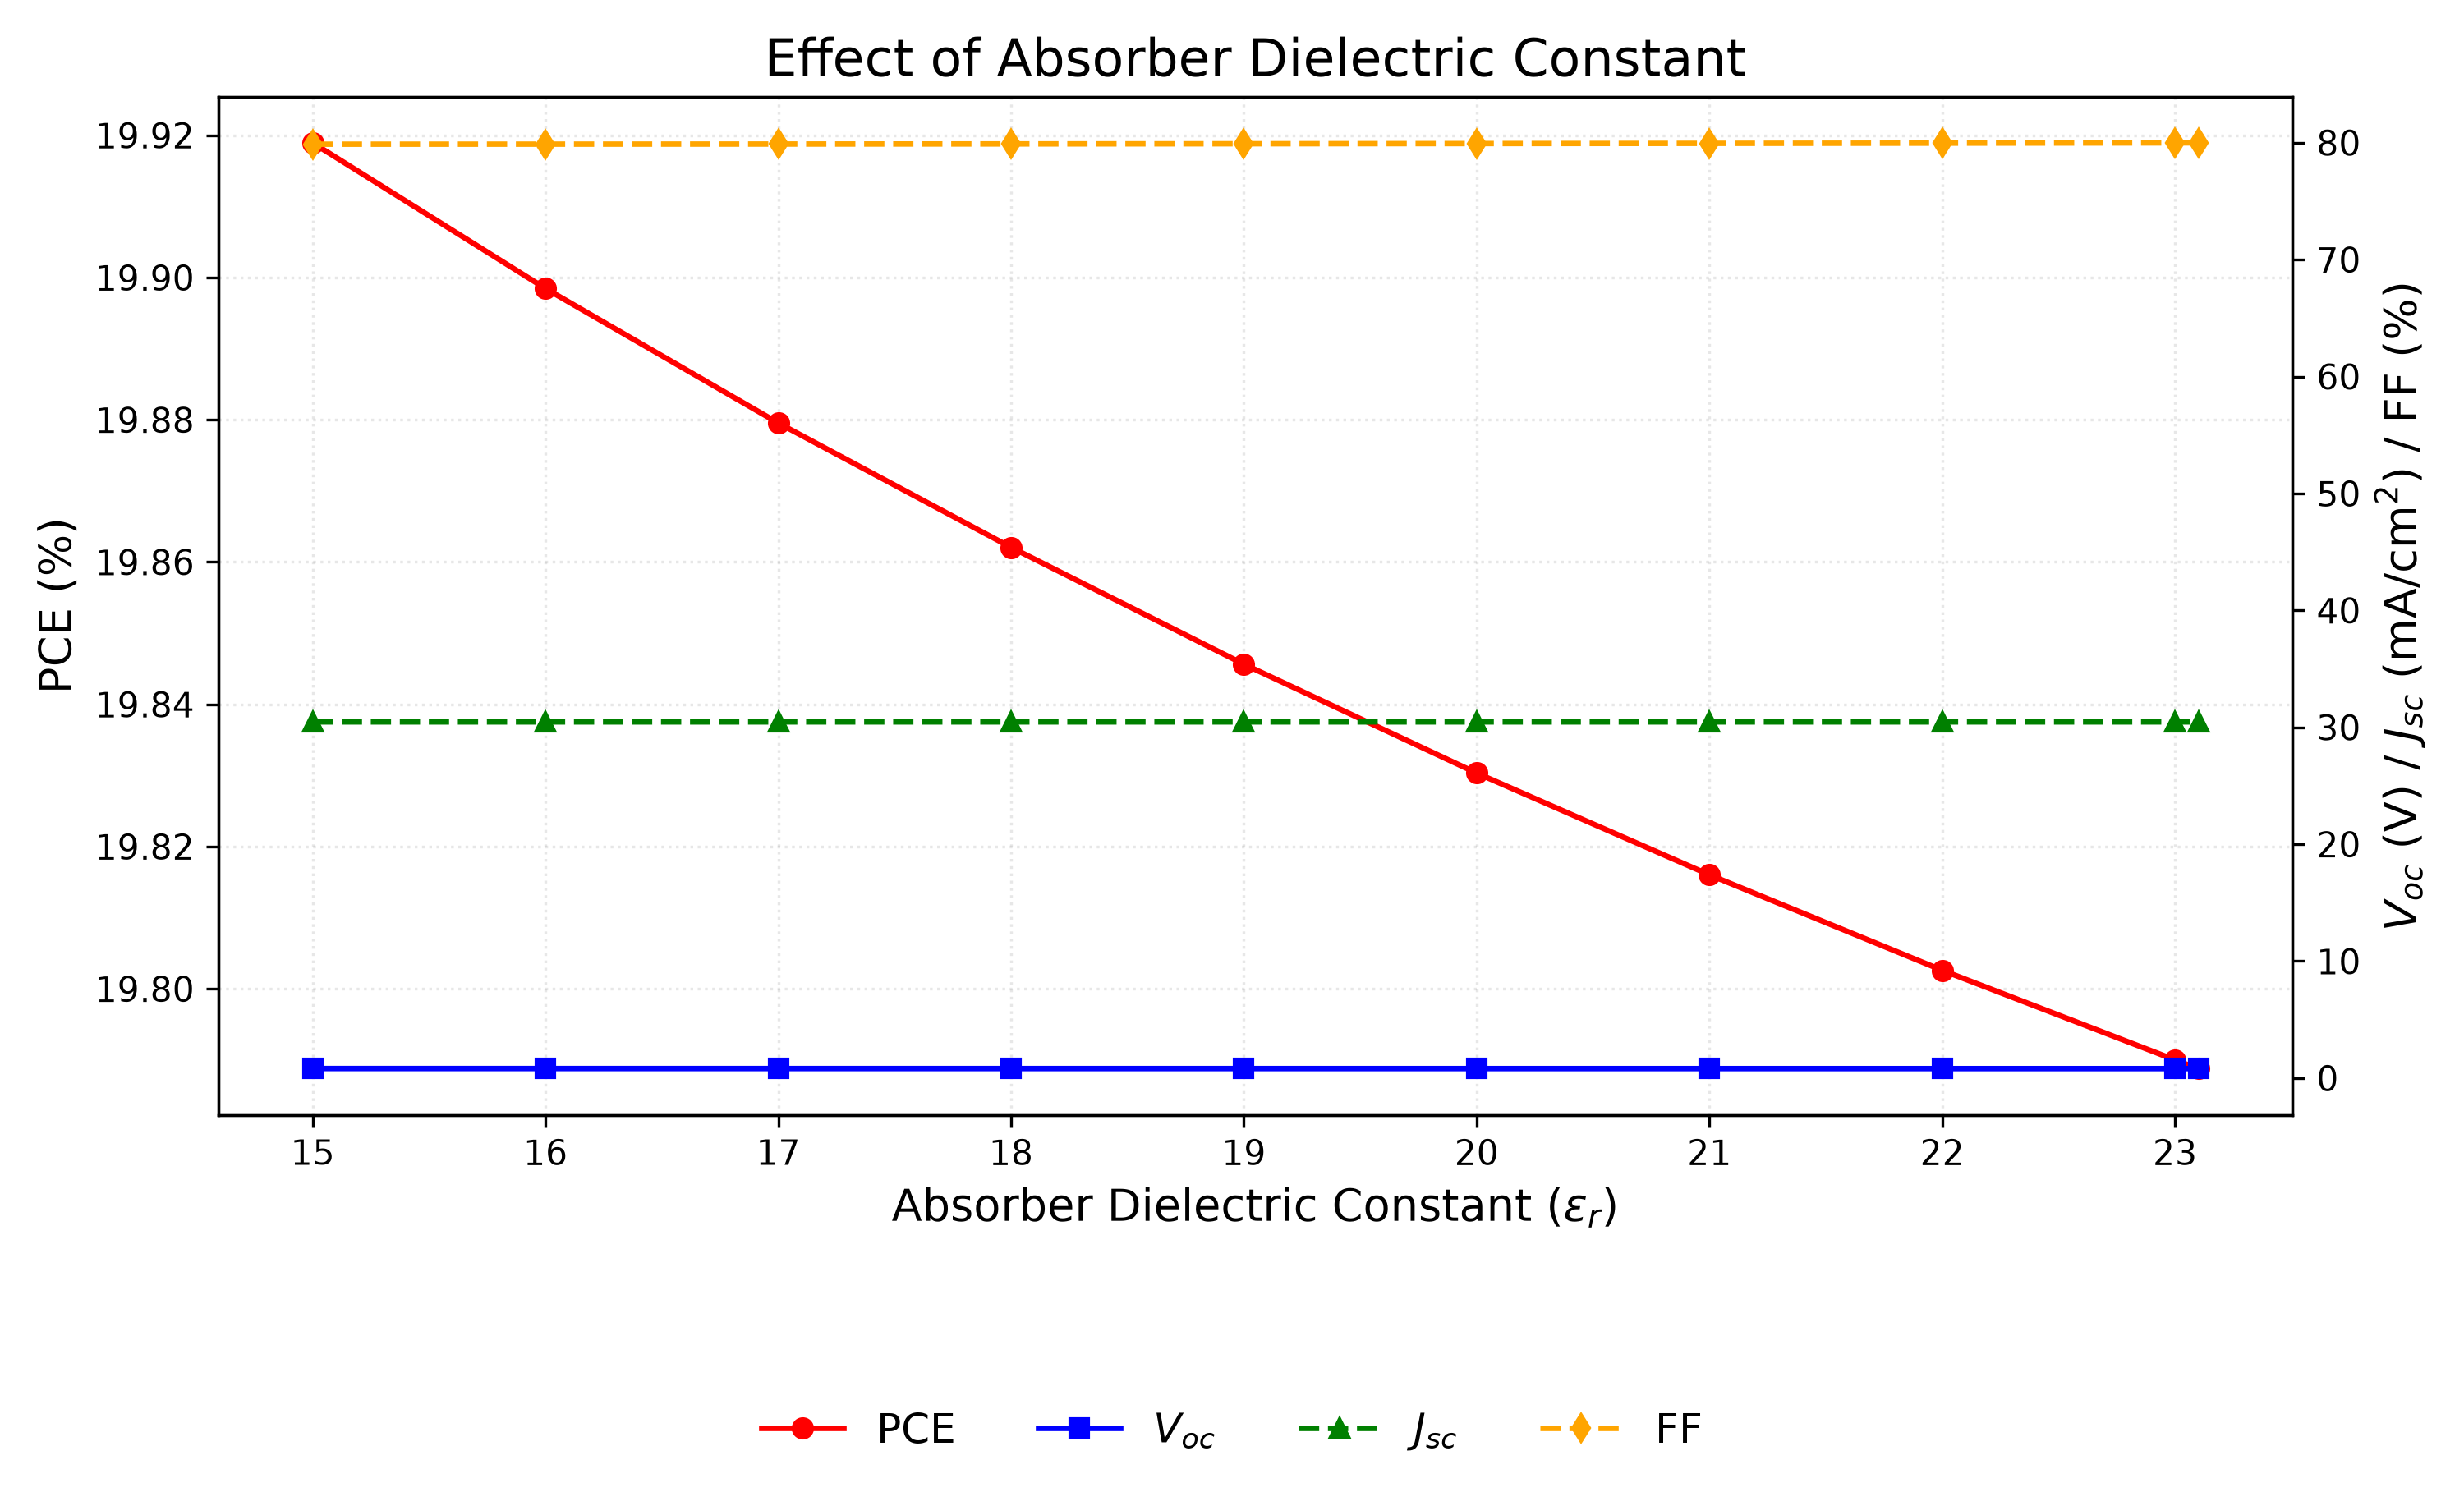
\includegraphics[width=0.85\linewidth]{figs/fig5.png}
\caption{Variation of PCE, V$_{\mathrm{OC}}$, J$_{\mathrm{SC}}$, and FF with RbGeI$_{3}$ absorber dielectric constant. The performance is essentially insensitive to $\epsilon$r across the investigated range; $\epsilon$r = 15 is used in the final device.}
\end{figure}

\subsection*{Effect of absorber electron affinity}
Electron affinity lines up the energy bands between adjacent layers and so controls extraction of the charge carriers. We held everything else fixed and stepped $\chi$ from 3.9 to 4.2 eV.
Peak performance lands at $\chi$ = 3.9 eV with a PCE of 19.79\%. Raise the affinity to 4.2 eV and V$_{\mathrm{OC}}$ falls from 0.812 to 0.710 V while J$_{\mathrm{SC}}$ holds flat: the extra electron affinity buys a fill-factor gain smaller than the voltage it costs. We stay at 3.9 eV.


\begin{figure}[htbp]
\centering
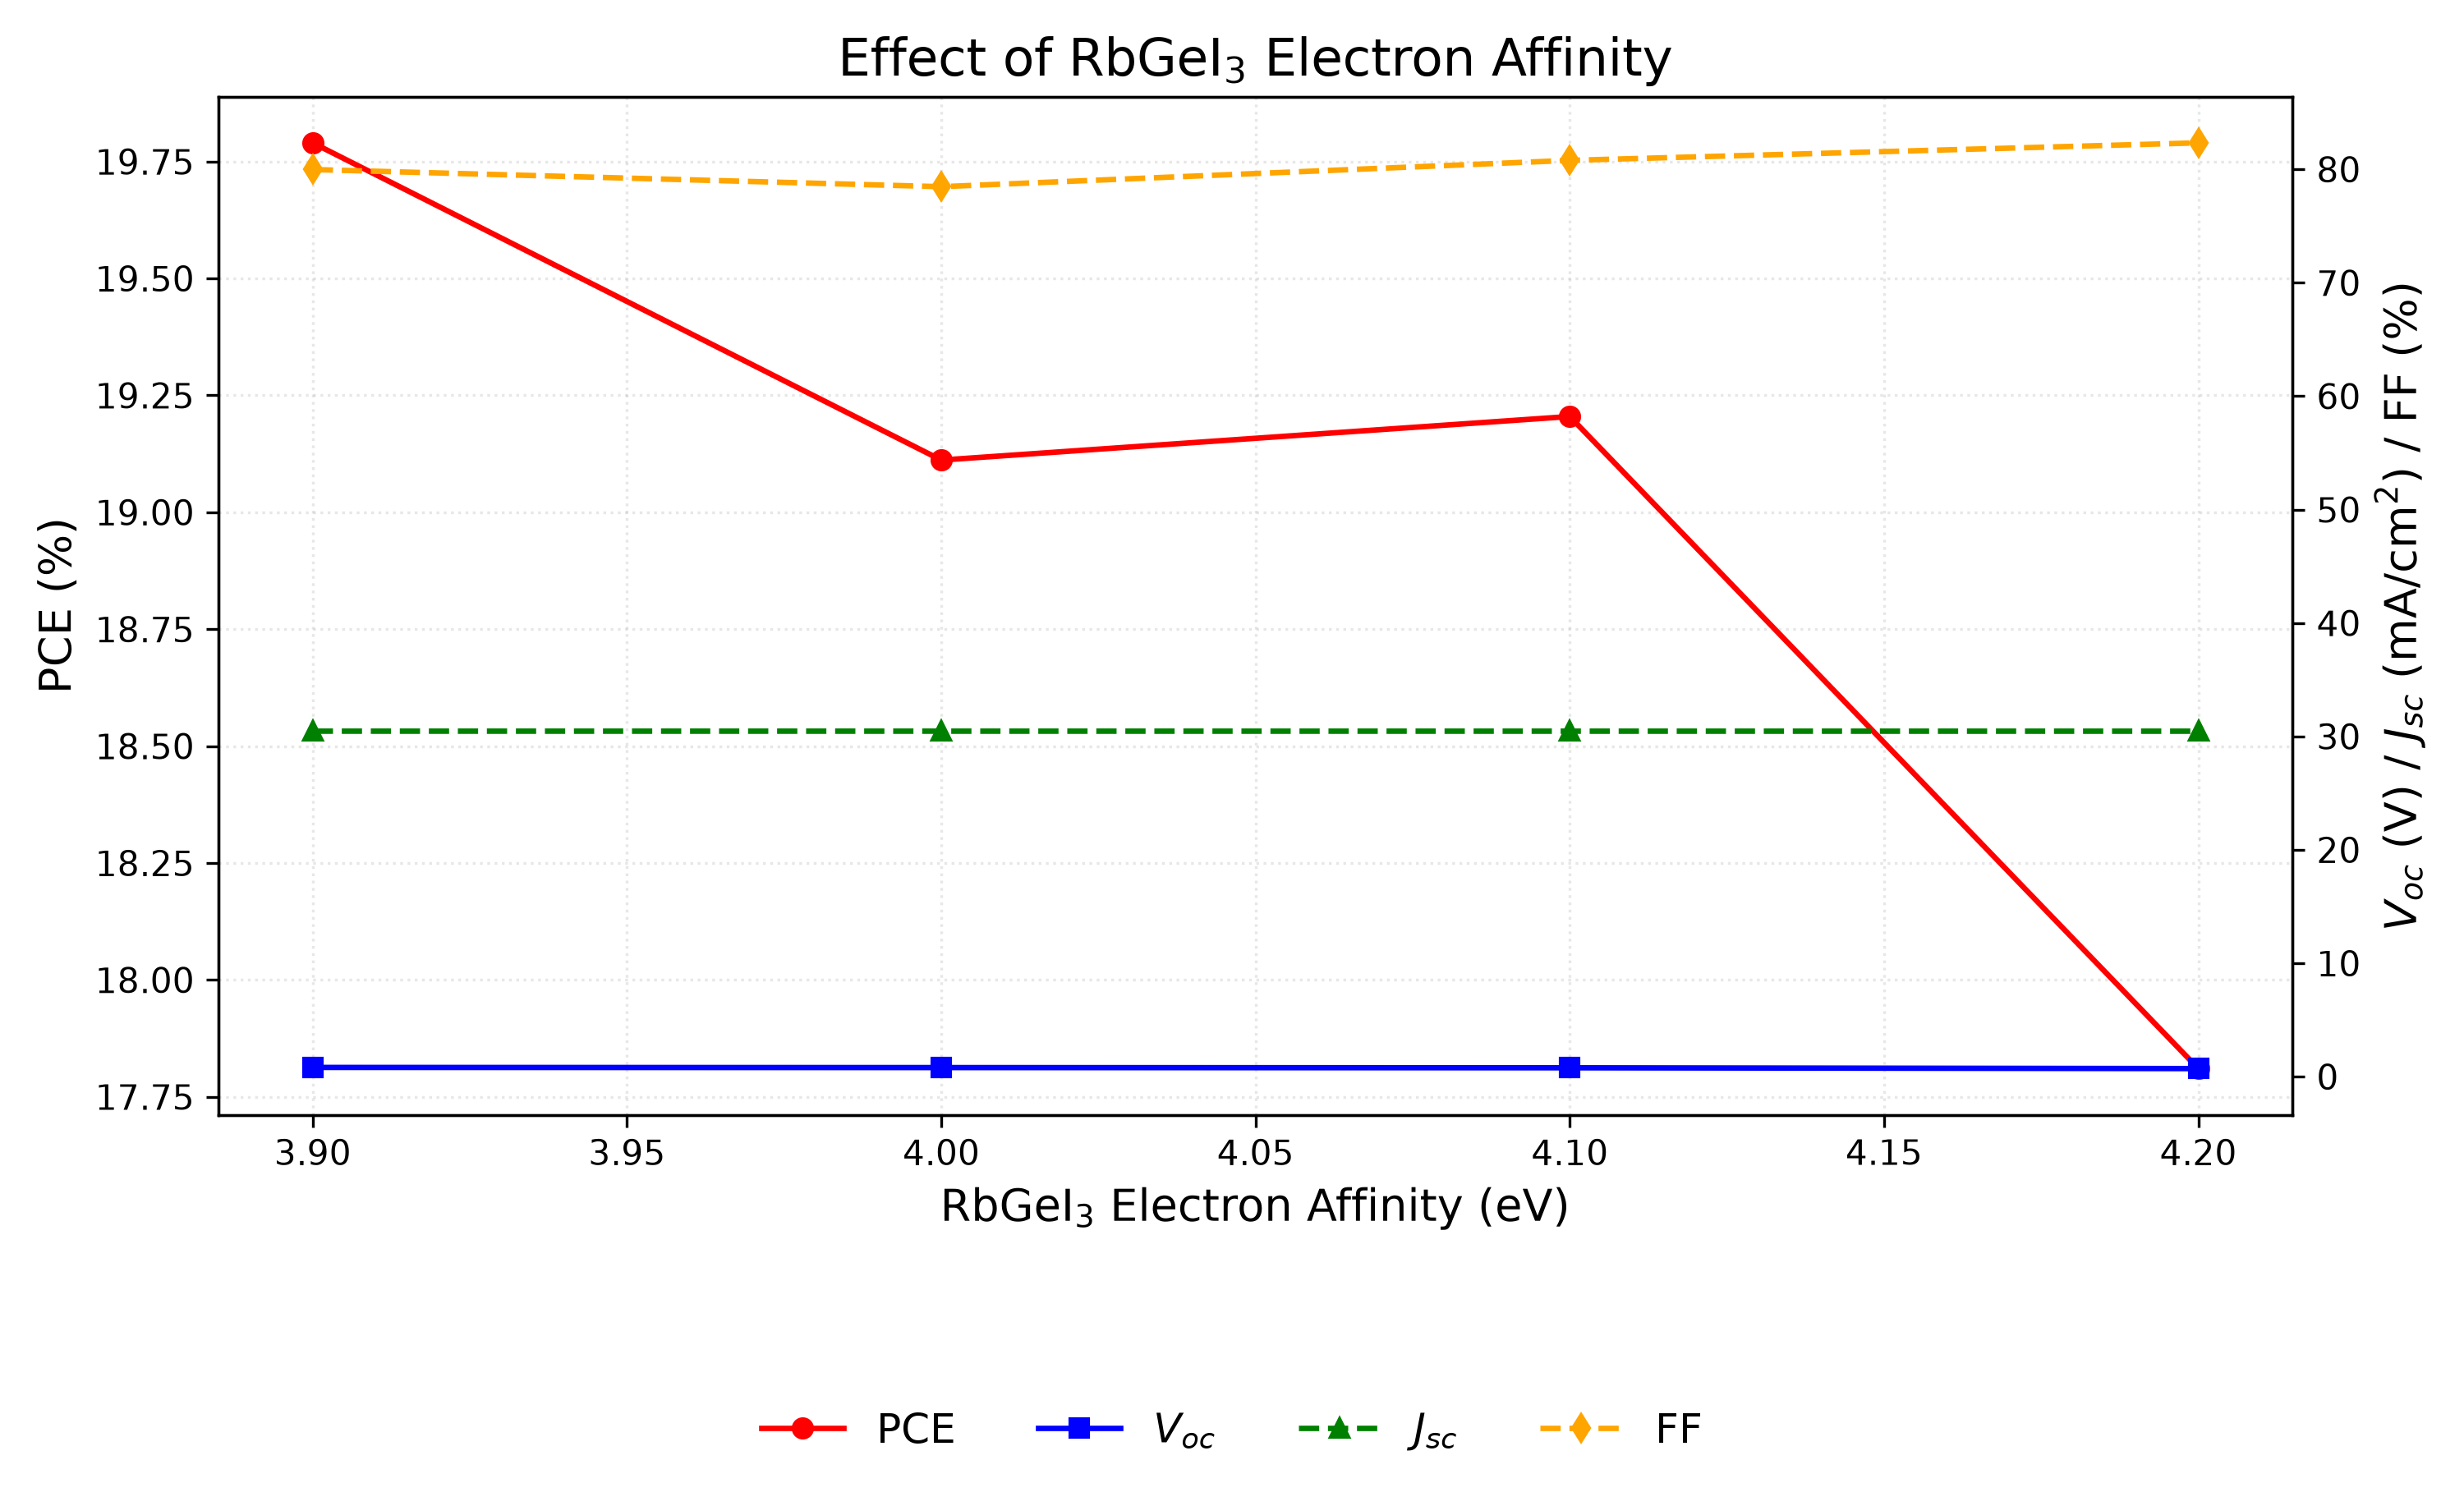
\includegraphics[width=0.85\linewidth]{figs/fig6.png}
\caption{Variation of PCE, V$_{\mathrm{OC}}$, J$_{\mathrm{SC}}$, and FF with RbGeI$_{3}$ absorber electron affinity. PCE is highest at $\chi$ = 3.9 eV due to optimal band alignment with TiO$_{2}$.}
\end{figure}

\subsection*{Effect of TiO$_{2}$/RbGeI$_{3}$ interfacial defect density}
The TiO$_{2}$/RbGeI$_{3}$ interface is where performance is won or lost. Varying its defect density from 10$^{12}$ to 10$^{18}$ cm$^{-2}$, with everything else fixed, sends the device off a cliff: PCE drops from 21.04\% to 8.40\%, V$_{\mathrm{OC}}$ from 0.827 to 0.439 V, J$_{\mathrm{SC}}$ from 30.46 to 28.09 mA/cm$^{2}$, and FF from 83.52\% to 68.11\% (Figure S4).
More states at the TiO$_{2}$/RbGeI$_{3}$ junction mean more carriers captured before they reach the electrodes; V$_{\mathrm{OC}}$, J$_{\mathrm{SC}}$, and FF fall together. Best performance comes at the unphysical 10$^{12}$ cm$^{-2}$ floor, but the final device targets 10$^{14}$ cm$^{-2}$, a density a real film can hit and keep: Ge$^{2+}$ oxidation and moisture sensitivity during preparation make anything below that hard to hold consistently. The figure also matches the bulk density chosen in Section V.C and the value comparable SCAPS studies of lead-free perovskites assume.


\begin{figure}[htbp]
\centering
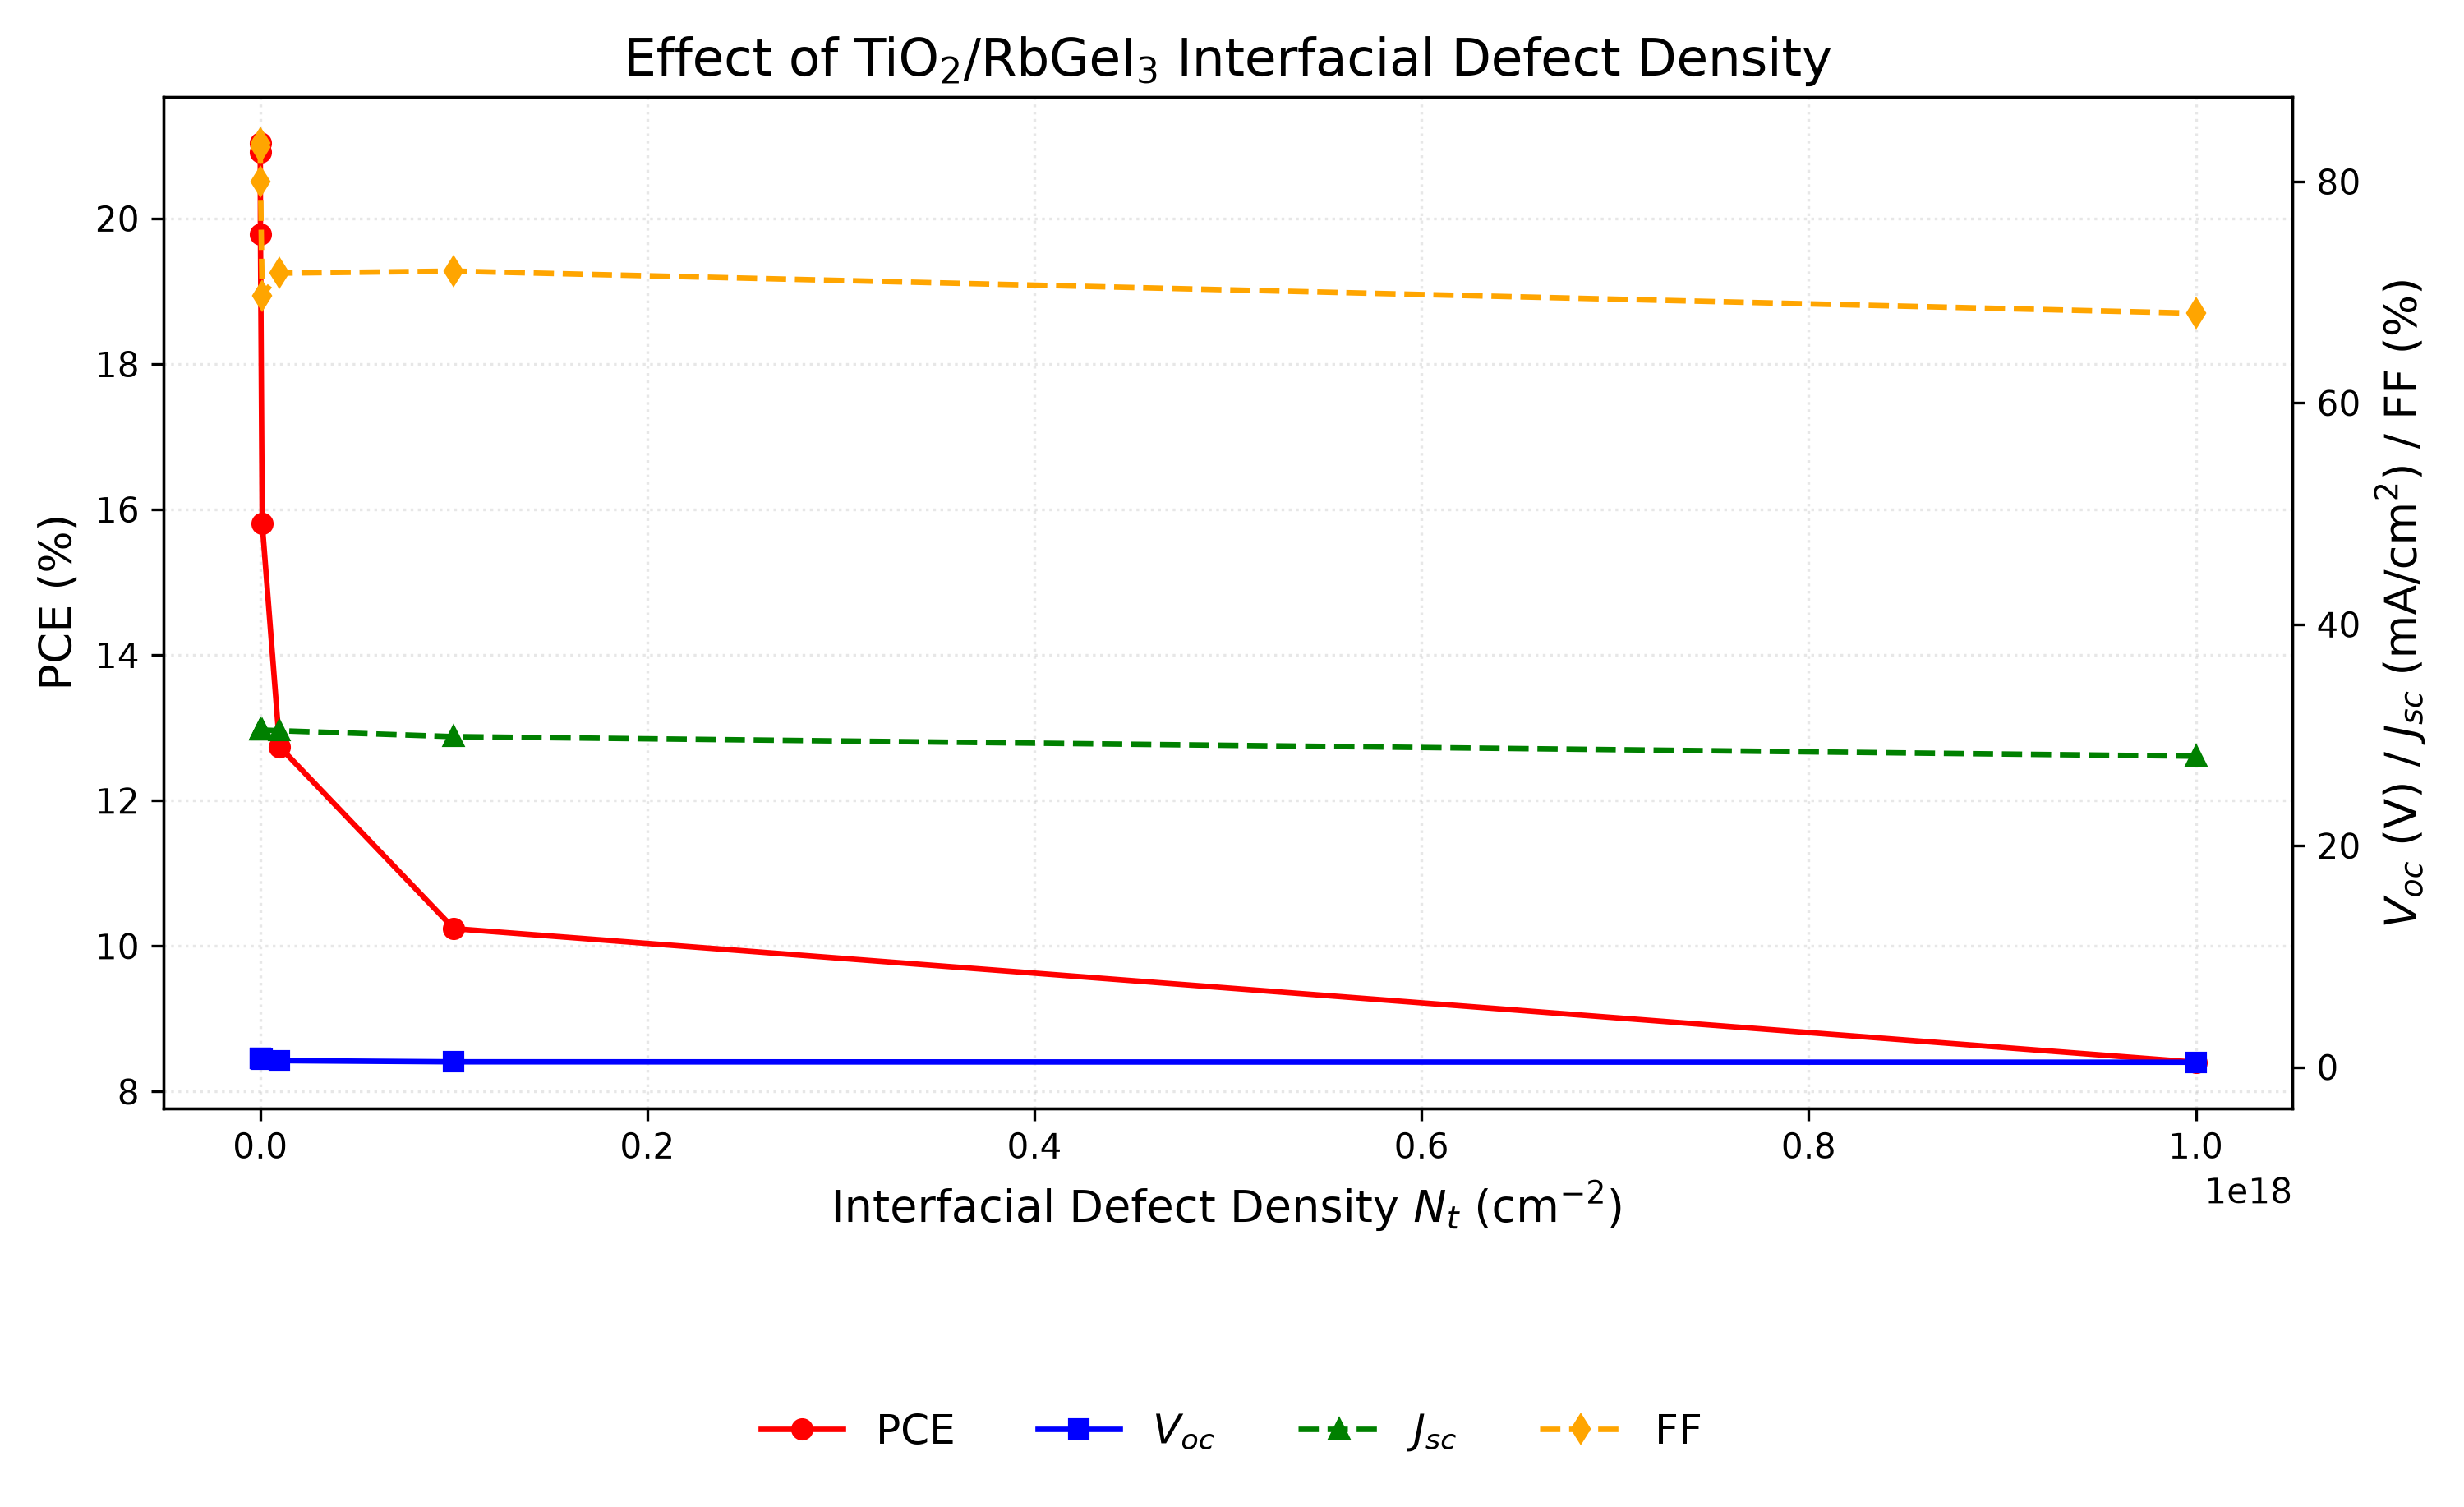
\includegraphics[width=0.85\linewidth]{figs/fig7.png}
\caption{Variation of PCE, V$_{\mathrm{OC}}$, J$_{\mathrm{SC}}$, and FF with TiO$_{2}$/RbGeI$_{3}$ interfacial defect density. Performance degrades sharply above 10$^{14}$ cm$^{-2}$; the RbGeI$_{3}$/CuI interface (Supplementary Section S1.5) is markedly more defect-tolerant.}
\end{figure}

\subsection*{Effect of RbGeI$_{3}$/CuI interfacial defect density}
The RbGeI$_{3}$/CuI junction is far more tolerant: PCE moves only from 19.79\% to 18.19\% across the same 10$^{12}$ to 10$^{18}$ cm$^{-2}$ range. That contrast pins the performance limit on the TiO$_{2}$/RbGeI$_{3}$ interface. The final device still adopts 10$^{14}$ cm$^{-2}$ here to match the electron side (Supplementary Section S1.4); the modest penalty is the price of internal consistency.


\begin{figure}[htbp]
\centering
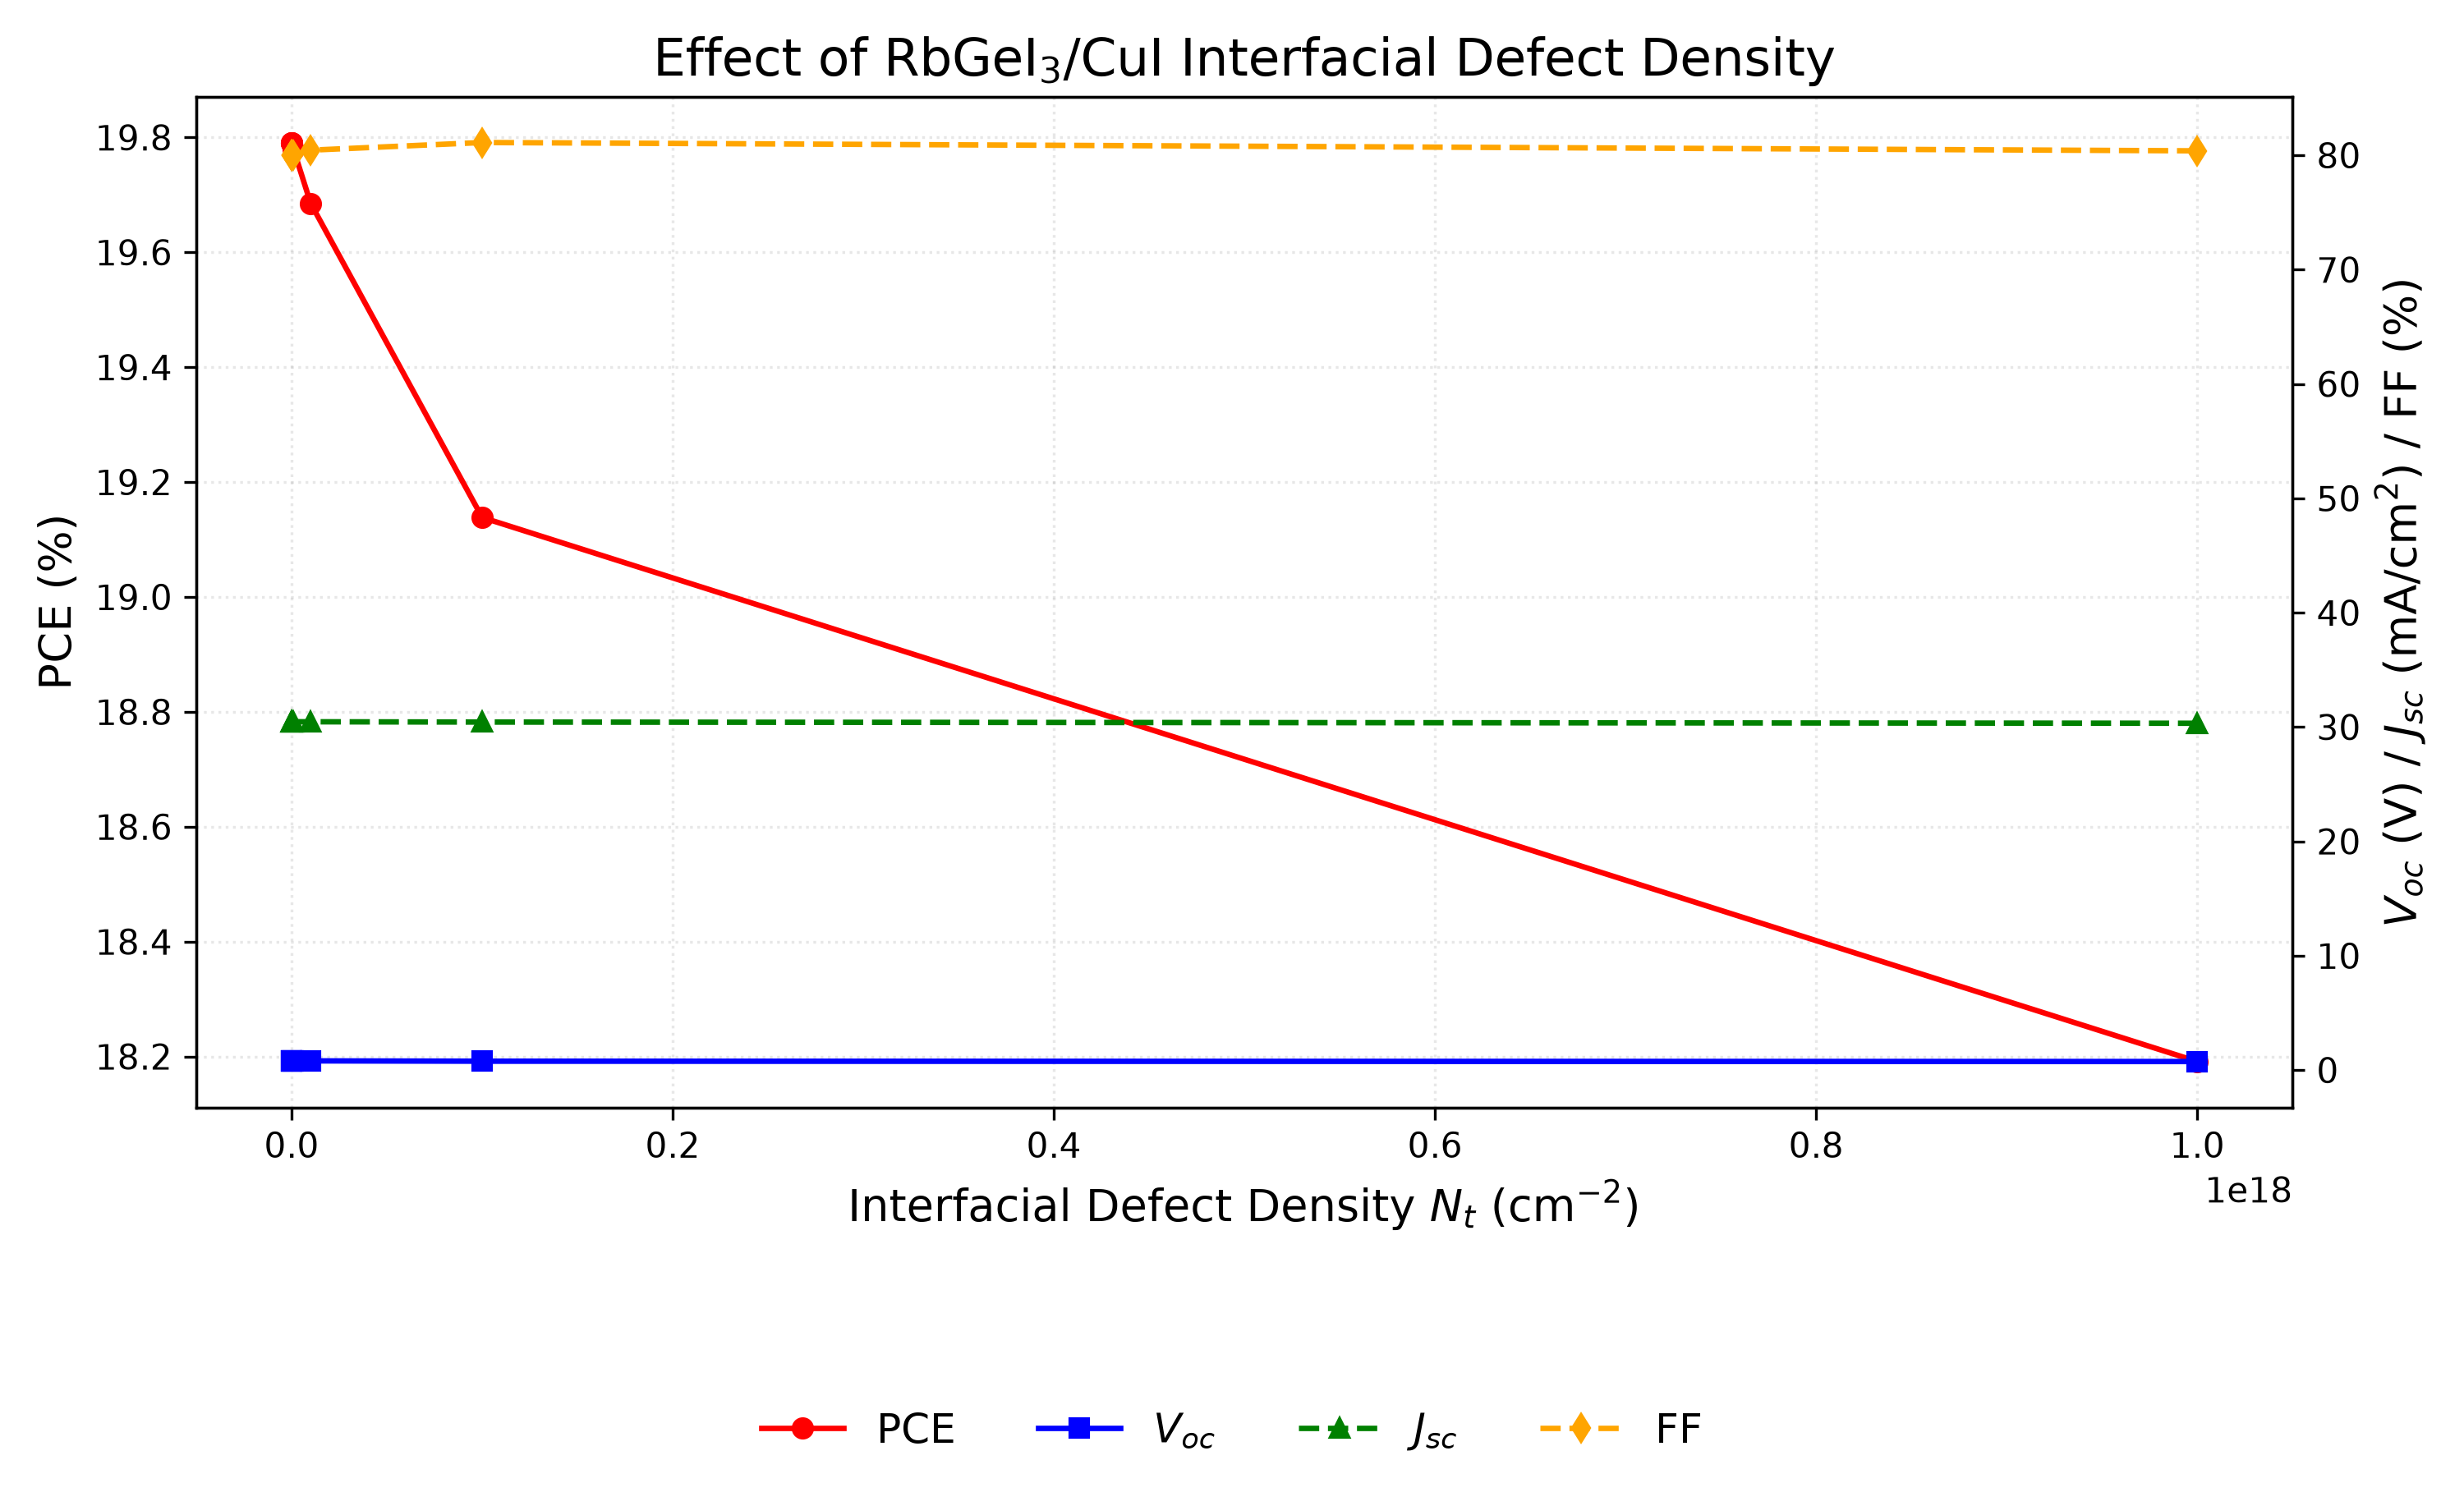
\includegraphics[width=0.85\linewidth]{figs/fig8.png}
\caption{Variation of PCE, V$_{\mathrm{OC}}$, J$_{\mathrm{SC}}$, and FF with RbGeI$_{3}$/CuI interfacial defect density. The interface is markedly more defect-tolerant than the TiO$_{2}$/RbGeI$_{3}$ interface; 10$^{14}$ cm$^{-2}$ is used here too.}
\end{figure}

\subsection*{Effect of absorber bandgap}
The bandgap picks which wavelengths the cell can use. Moving it from 1.3 to 1.7 eV, all else constant, raises Voc from 0.840 V to 1.002 V as expected from larger quasi-Fermi-level splitting, while Jsc falls from 33.59 to 20.30 mA/cm$^{2}$ because a wider gap throws away more of the spectrum.
The maximum thus sits at 1.4 eV, within 0.06 eV of the Shockley--Queisser (SQ) optimum of $\approx$1.34 eV for a single junction \cite{r35,r36,r37}, so the absorber runs at 1.4 eV; tabulated SQ limits imply an ideal J$_{\mathrm{SC}}$ of $\approx$33 mA/cm$^{2}$ and a maximum efficiency of $\approx$33\% at this bandgap \cite{r36}. On both sides of the SQ optimum the limiting efficiency declines, steeply for wider bandgaps because fewer photons are absorbed \cite{r36,r37}: a 2.0 eV absorber would shift its absorption edge to $\lambda$c $\approx$ 620 nm and exclude most of the visible spectrum, and our sweep already shows J$_{\mathrm{SC}}$ falling to 20.30 mA/cm$^{2}$ at 1.7 eV, whereas at 1.3 eV the higher J$_{\mathrm{SC}}$ (33.59 mA/cm$^{2}$) does not offset the V$_{\mathrm{OC}}$ loss (0.840 V). The corresponding cutoff wavelength is $\lambda$c = 1240 / 1.4 $\approx$ 886 nm, consistent with the absorption edge observed in the quantum-efficiency spectrum of Section V.D of the main text. A targeted re-simulation varying only the absorption-grading endpoints (graded 885.7--1033.3 nm versus flat 885.7--885.7 nm, all else fixed) changes J$_{\mathrm{SC}}$ by 0.00 mA/cm$^{2}$, and the consolidated J$_{\mathrm{SC}}$ of 30.32 mA/cm$^{2}$ lies below the SQ limit of $\approx$33 mA/cm$^{2}$ at 1.4 eV, so the headline result is admissible with uniform square-root-law absorption at the electrical bandgap; the 26.81\% device is therefore reported as an ideal-coupling upper bound, with a quantified realistic window given in Sections V.G and VII.A of the main text.


\begin{figure}[htbp]
\centering
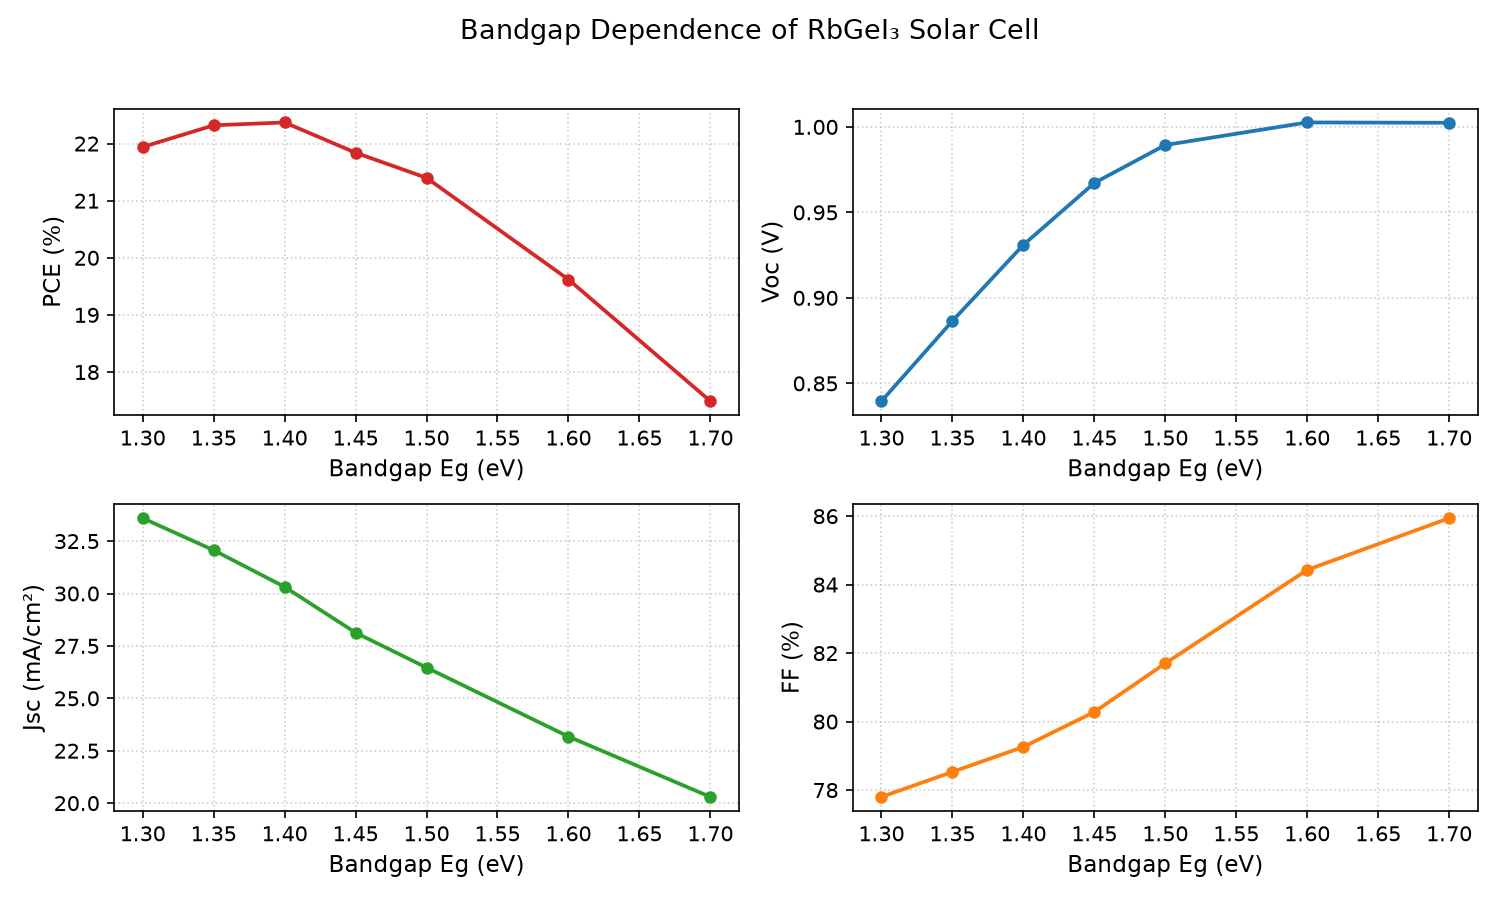
\includegraphics[width=0.85\linewidth]{figs/fig9.png}
\caption{Variation of PCE, V$_{\mathrm{OC}}$, J$_{\mathrm{SC}}$, and FF with RbGeI$_{3}$ absorber bandgap. PCE peaks at 1.4 eV, close to the Shockley--Queisser optimum.}
\end{figure}

\subsection*{Effect of TiO$_{2}$ ETL thickness}
Thickness of the TiO$_{2}$ ETL cuts across electron extraction, transport, and optical transmission at once. Sweeping it from 0.01 to 0.09 $\mu$m, all else fixed, gives the best PCE at the thinnest layers: 21.12\% at 10 nm, a local low of 18.72\% at 0.04 $\mu$m, and a partial recovery to 19.97\% at 0.09 $\mu$m. Planar SCAPS studies stick to thin ($\leq$50 nm) ETLs for the same reason we do: thicker ones add series resistance and soak up photons.


\begin{figure}[htbp]
\centering
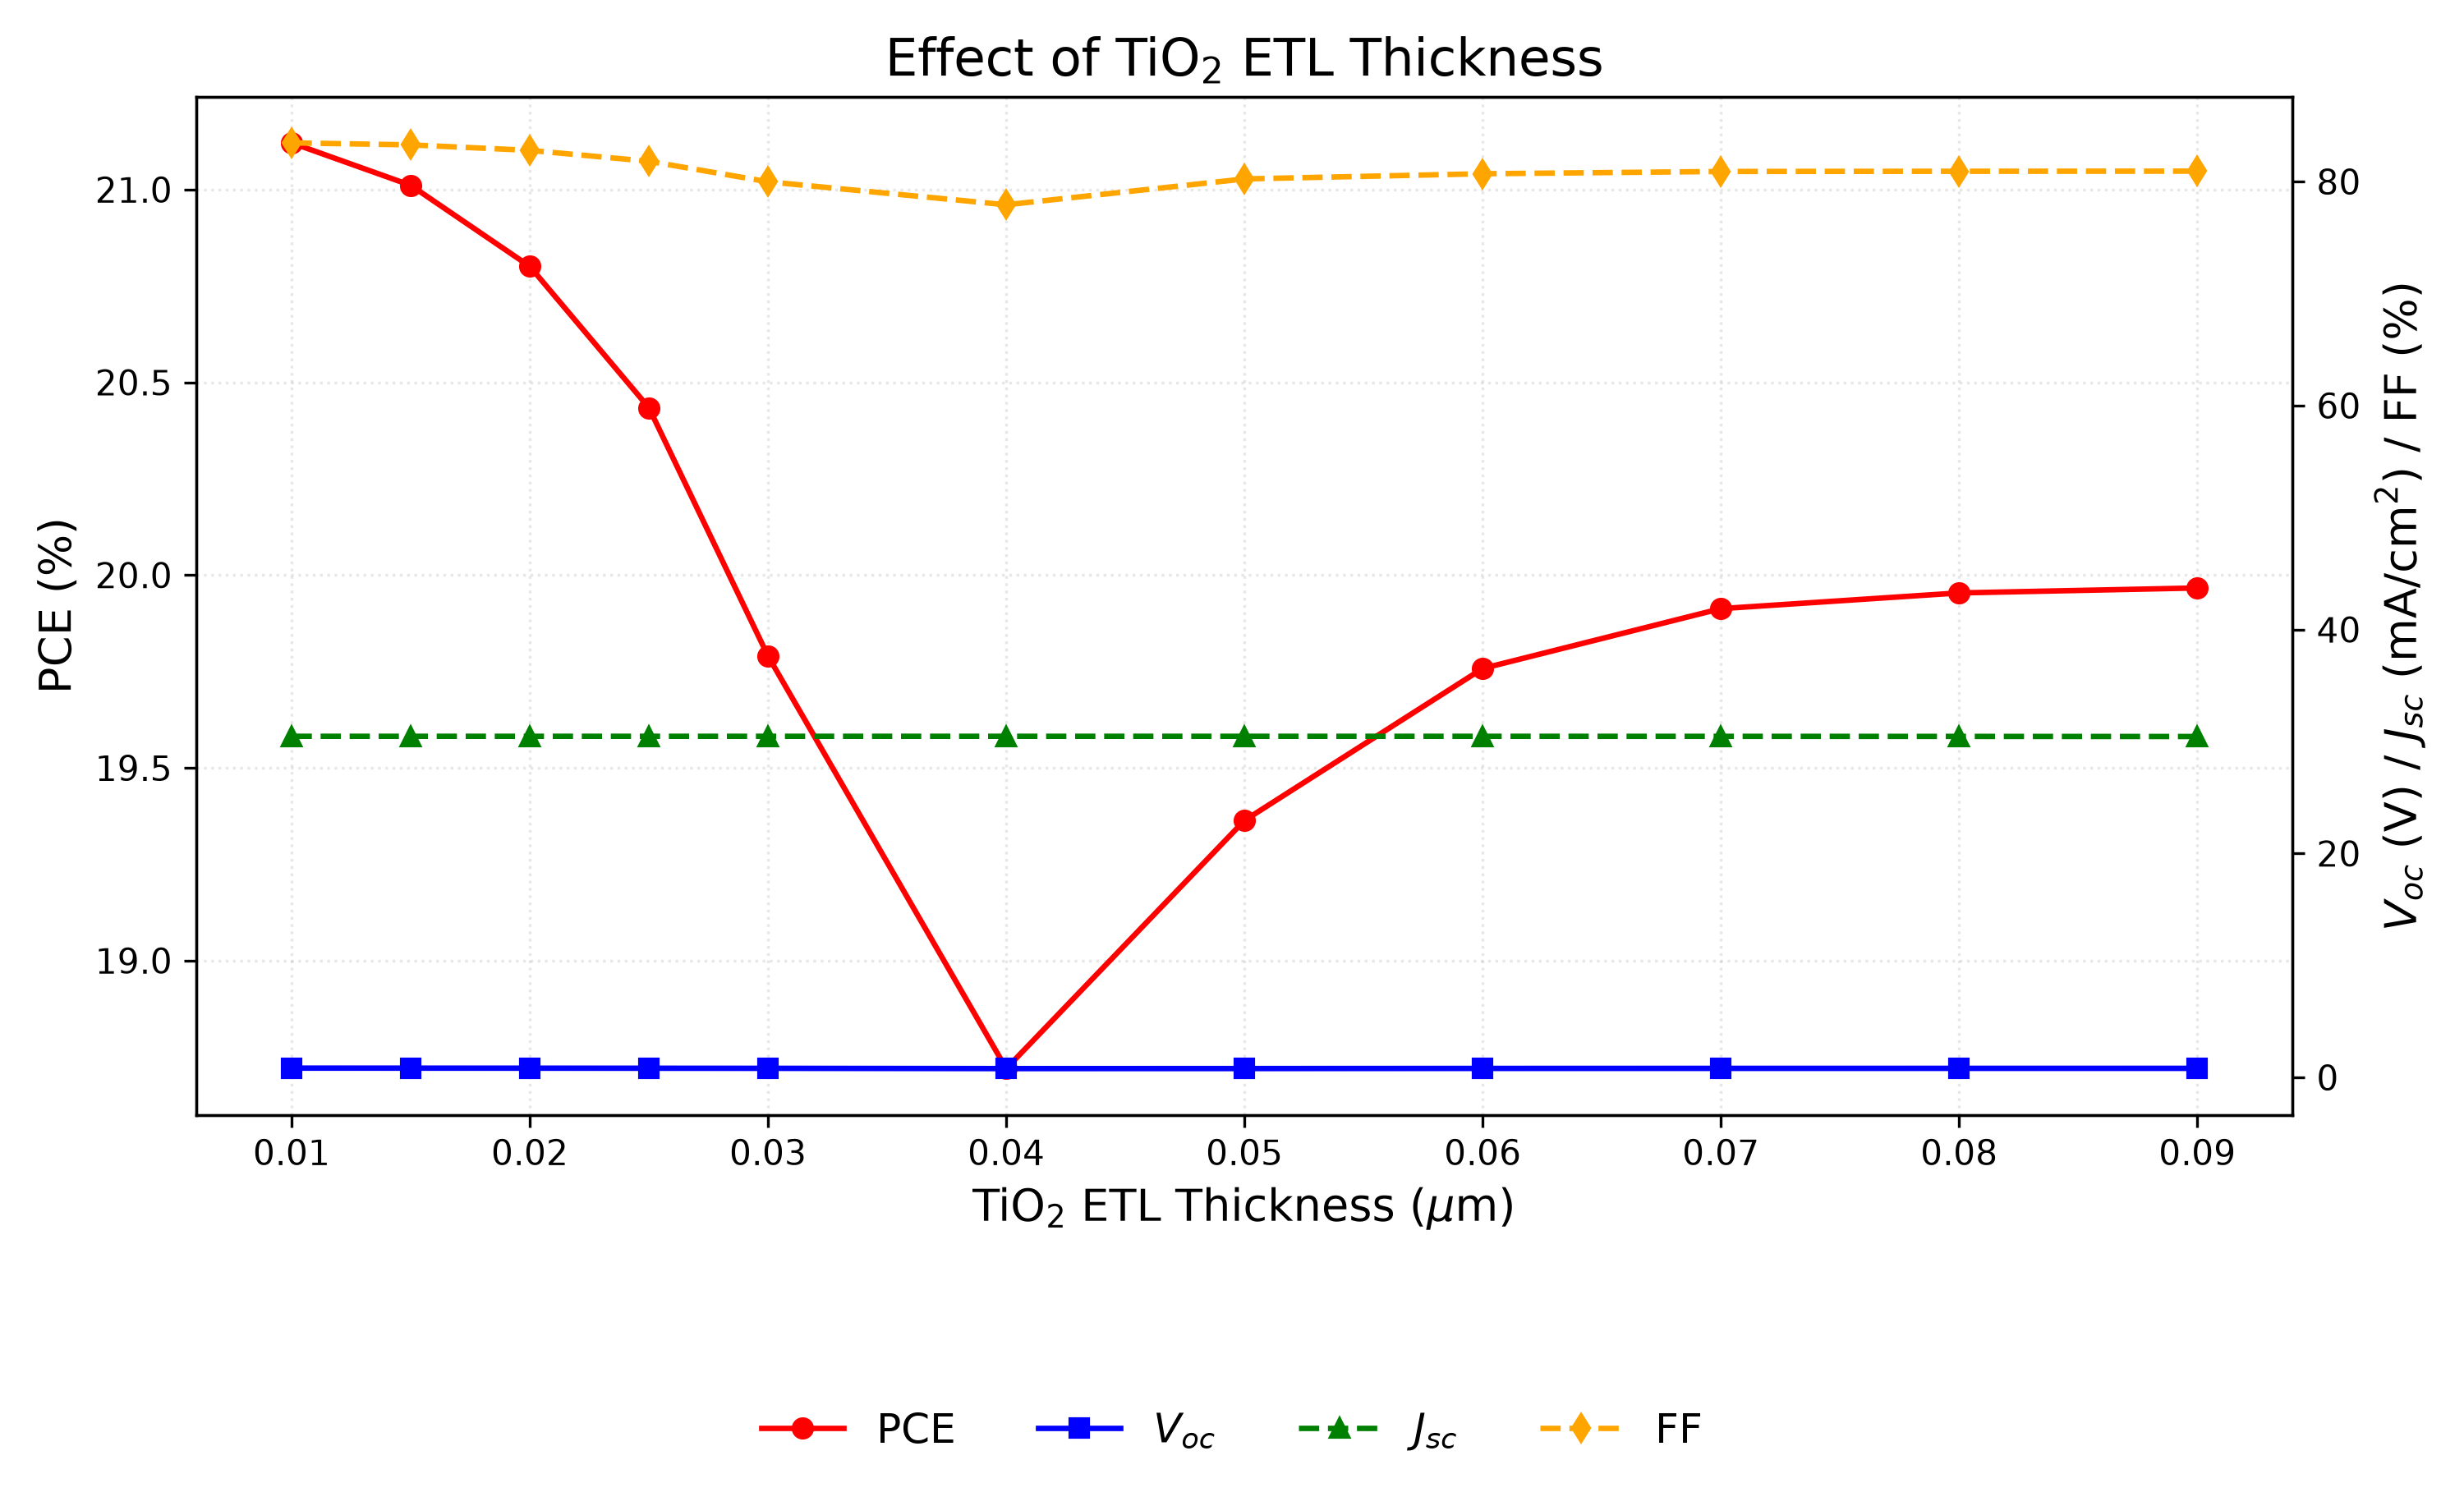
\includegraphics[width=0.85\linewidth]{figs/fig10.png}
\caption{Variation of PCE, V$_{\mathrm{OC}}$, J$_{\mathrm{SC}}$, and FF with TiO$_{2}$ ETL thickness. PCE is highest at the thinnest ETL (10 nm), reflecting the shorter electron transport path.}
\end{figure}

\subsection*{Effect of CuI HTL thickness}
CuI thickness, swept from 0.1 to 1.9 $\mu$m, moves PCE by less than 0.002 percentage points; V$_{\mathrm{OC}}$, J$_{\mathrm{SC}}$, and FF stay essentially constant. That flatness lets us pick 100 nm purely to minimize material use. It sits at the low end of the 0.1--1.0 $\mu$m range comparable studies explored, which also reported a weak dependence.


\begin{figure}[htbp]
\centering
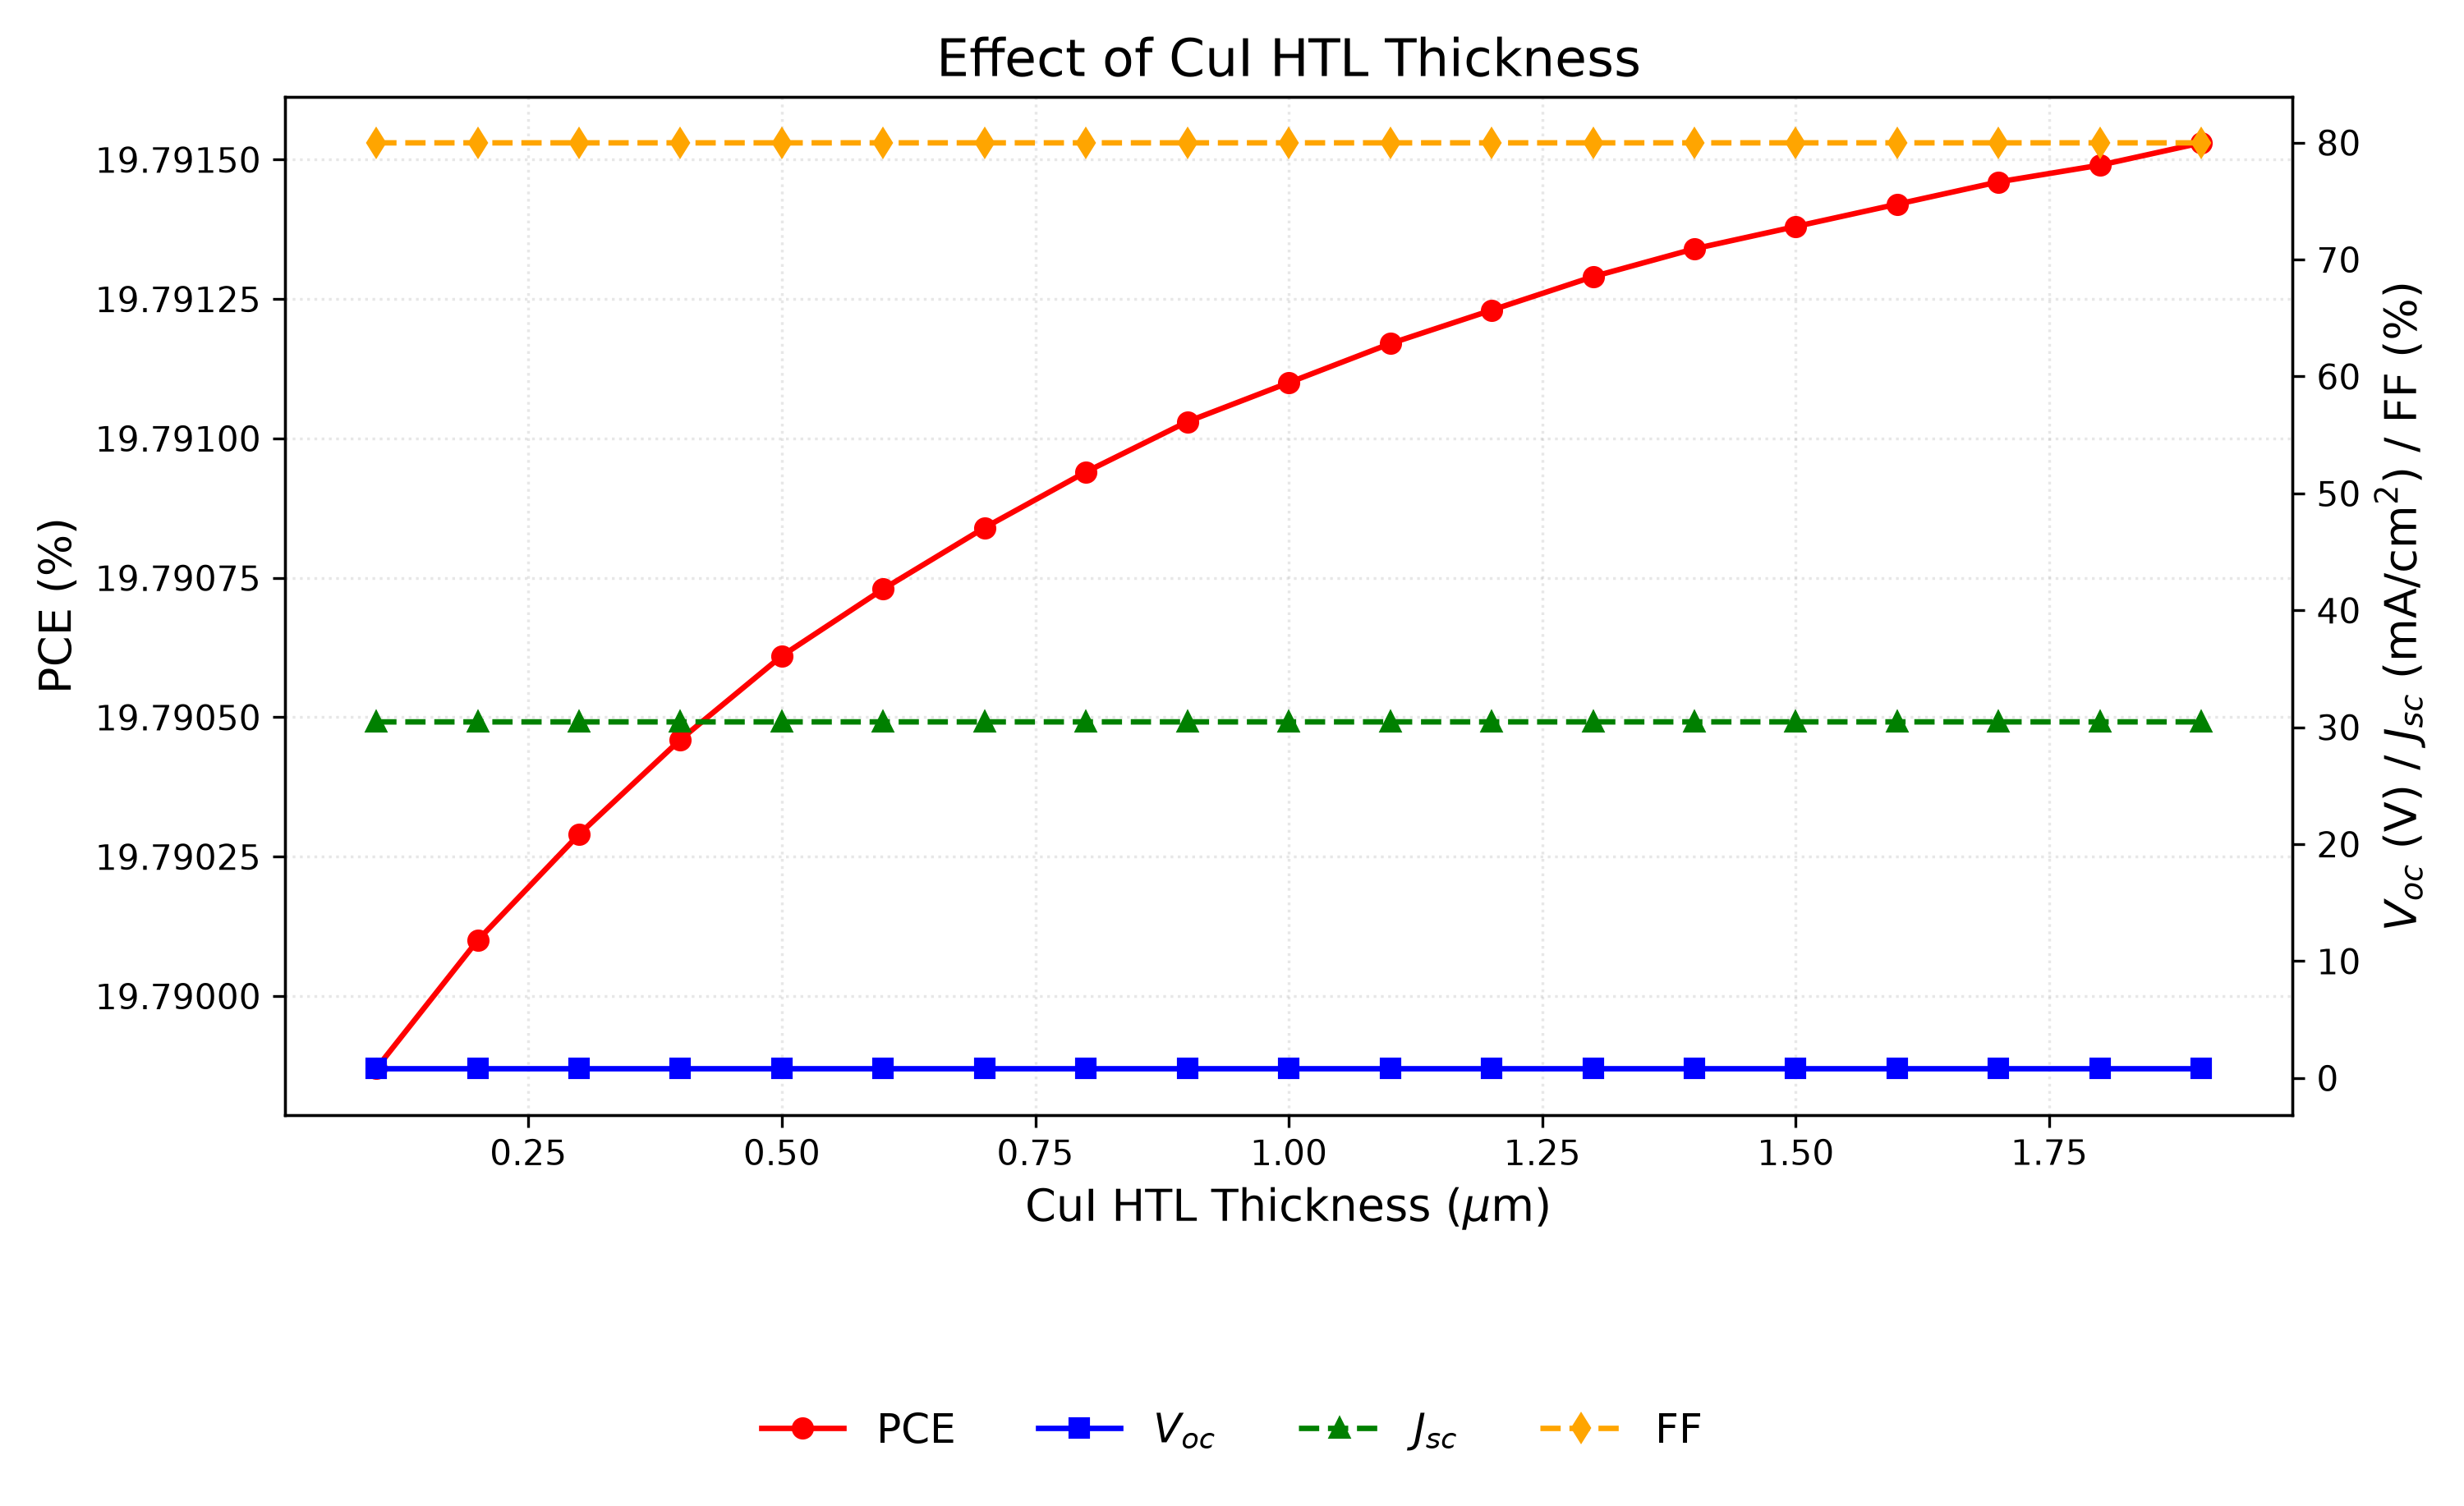
\includegraphics[width=0.85\linewidth]{figs/fig11.png}
\caption{Variation of PCE, V$_{\mathrm{OC}}$, J$_{\mathrm{SC}}$, and FF with CuI HTL thickness. The performance is essentially independent of HTL thickness; 100 nm minimizes material usage.}
\end{figure}

\subsection*{Effect of conduction-band effective density of states N$_{\mathrm{C}}$}
Raising N$_{\mathrm{C}}$ from 1$\times$10$^{17}$ to 1$\times$10$^{20}$ cm$^{-3}$ pushes PCE monotonically down from 20.65\% to 18.15\%; V$_{\mathrm{OC}}$ carries the loss (0.859 to 0.764 V) while J$_{\mathrm{SC}}$ barely stirs at $\sim$30.46 mA/cm$^{2}$. A lower N$_{\mathrm{C}}$ means a lower intrinsic carrier density and therefore a higher V$_{\mathrm{OC}}$, so the bottom of the sweep, 1$\times$10$^{17}$ cm$^{-3}$, goes into the final device. SCAPS studies commonly assume $\approx$10$^{18}$ cm$^{-3}$ for lead-free absorbers; we find going lower helps.


\begin{figure}[htbp]
\centering
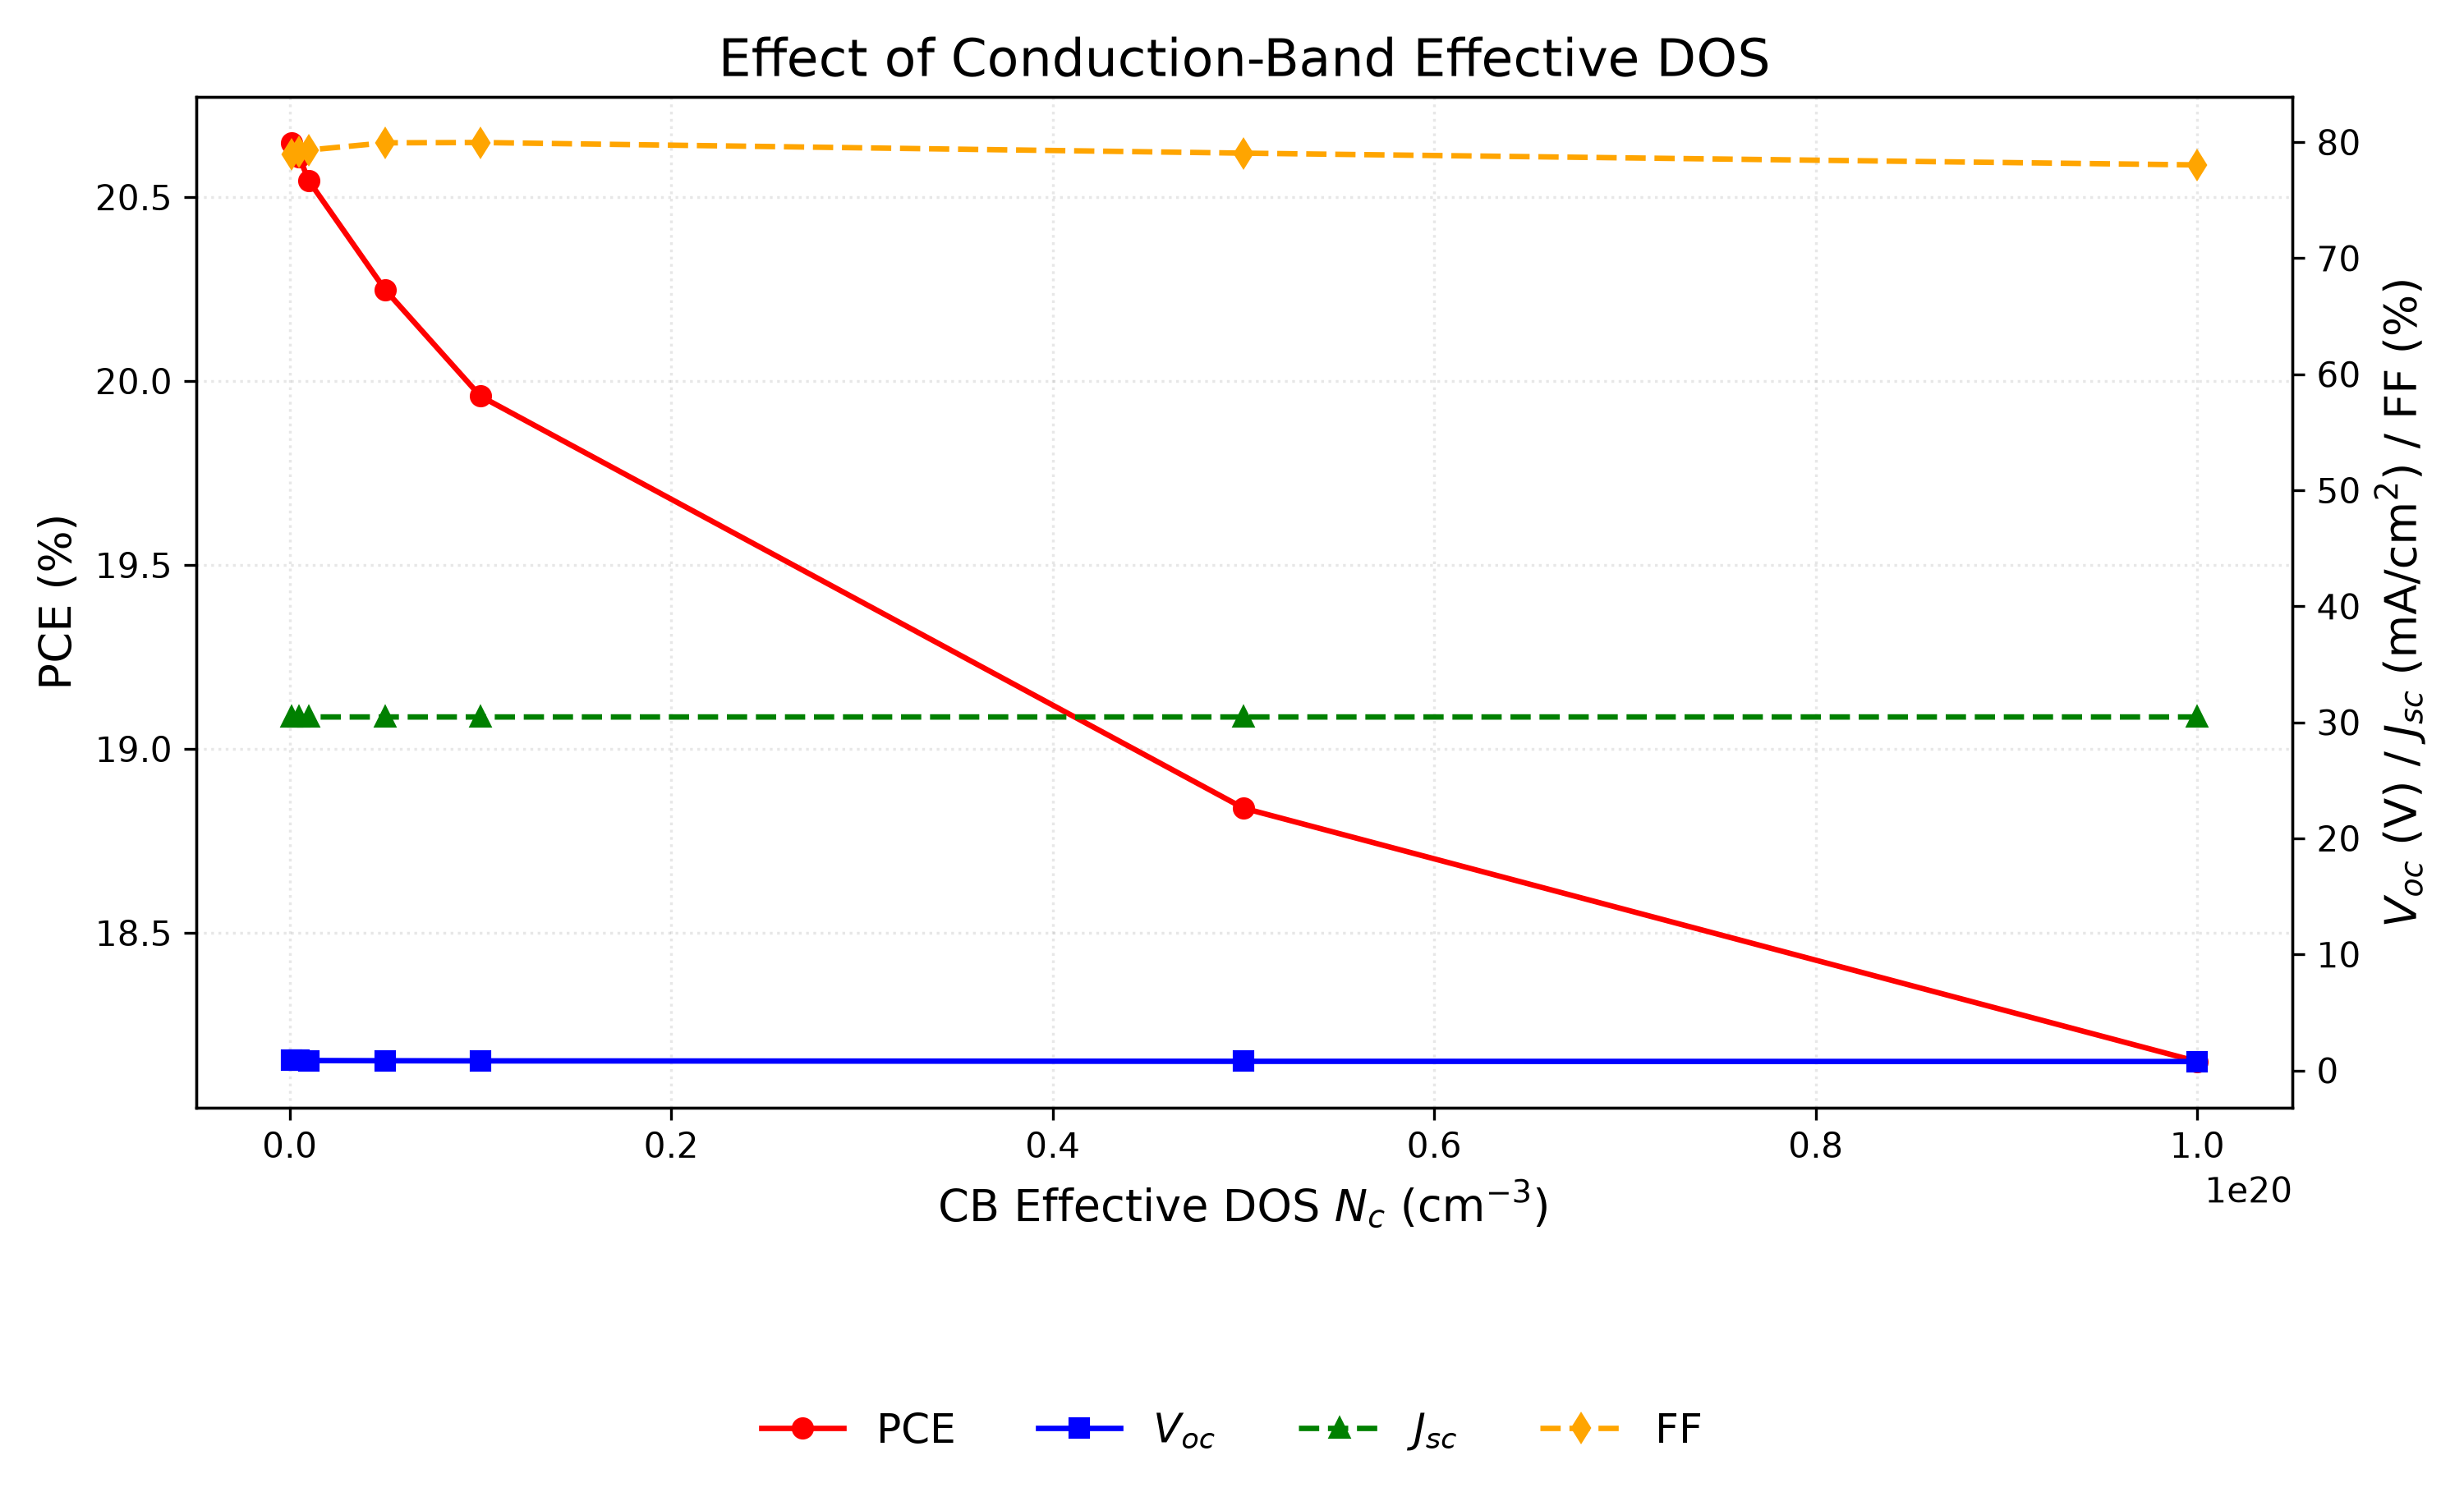
\includegraphics[width=0.85\linewidth]{figs/fig12.png}
\caption{Variation of PCE, V$_{\mathrm{OC}}$, J$_{\mathrm{SC}}$, and FF with conduction-band effective density of states N$_{\mathrm{C}}$. Lower N$_{\mathrm{C}}$ is preferred; the best value is 10$^{17}$ cm$^{-3}$.}
\end{figure}

\subsection*{Effect of valence-band effective density of states N$_{\mathrm{V}}$}
N$_{\mathrm{V}}$ behaves like N$_{\mathrm{C}}$ but hits harder. Across 1$\times$10$^{17}$ to 1$\times$10$^{20}$ cm$^{-3}$, PCE drops from 23.54\% to 18.86\% as V$_{\mathrm{OC}}$ slides from 0.945 to 0.780 V with J$_{\mathrm{SC}}$ flat. The smallest value wins again: N$_{\mathrm{V}}$ = 1$\times$10$^{17}$ cm$^{-3}$ is carried into the final set.


\begin{figure}[htbp]
\centering
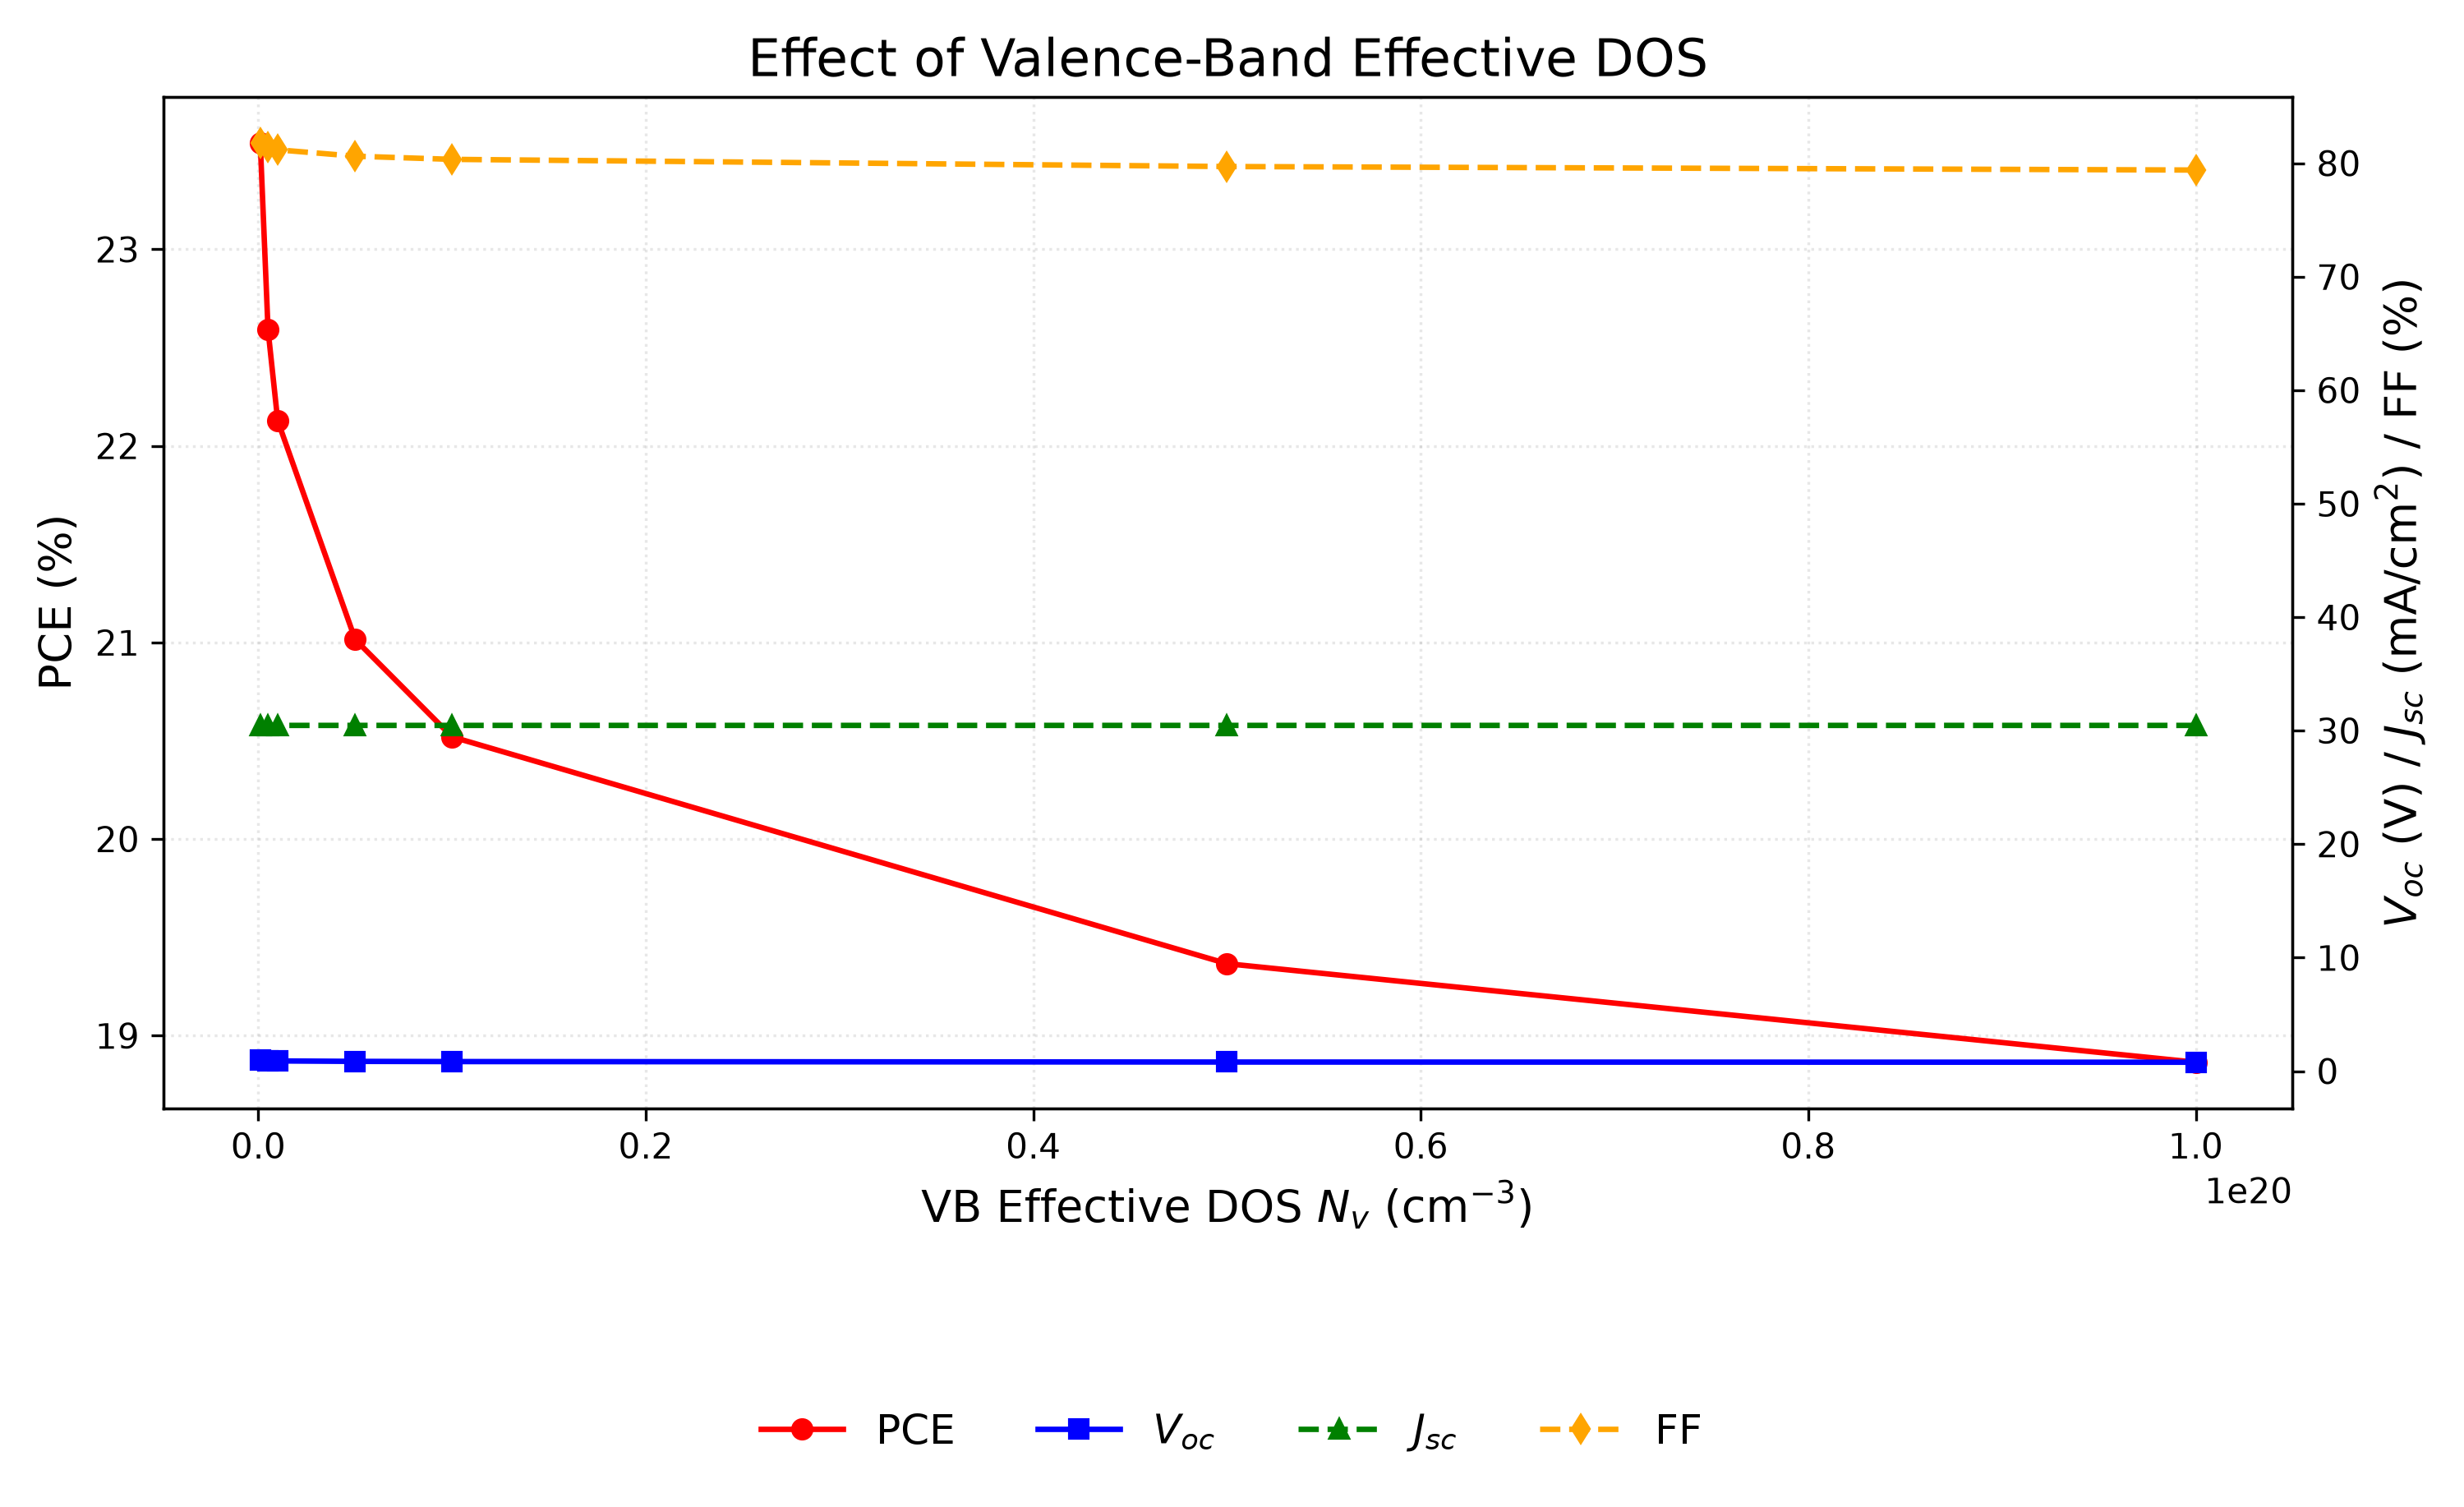
\includegraphics[width=0.85\linewidth]{figs/fig13.png}
\caption{Variation of PCE, V$_{\mathrm{OC}}$, J$_{\mathrm{SC}}$, and FF with valence-band effective density of states N$_{\mathrm{V}}$. The effect is more pronounced than for N$_{\mathrm{C}}$; the best value is 10$^{17}$ cm$^{-3}$.}
\end{figure}

\section*{S2.\ Illumination and dark characteristics}
\subsection*{Illumination dependence}
The optimized cell was also driven under 0.1 to 1.5 suns (Figure S11). J$_{\mathrm{SC}}$ tracks intensity almost linearly, the natural consequence of carrier generation scaling with photon flux, while V$_{\mathrm{OC}}$ rises logarithmically. The slope of that logarithmic rise gives an ideality factor n $\approx$ 1.17, so deep-defect Shockley-Read-Hall recombination is not dominant under operating conditions, and the cell stays efficient across the entire range. Re-simulation (0.1--1.5 suns, archived illum\_results.json) gives J$_{\mathrm{SC}}$ = 30.32 $\times$ suns + 0.00 (perfect linearity) and n = 1.17 from the V$_{\mathrm{OC}}$--ln(I) slope, confirming the reported n $\approx$ 1.2.


\begin{figure}[htbp]
\centering
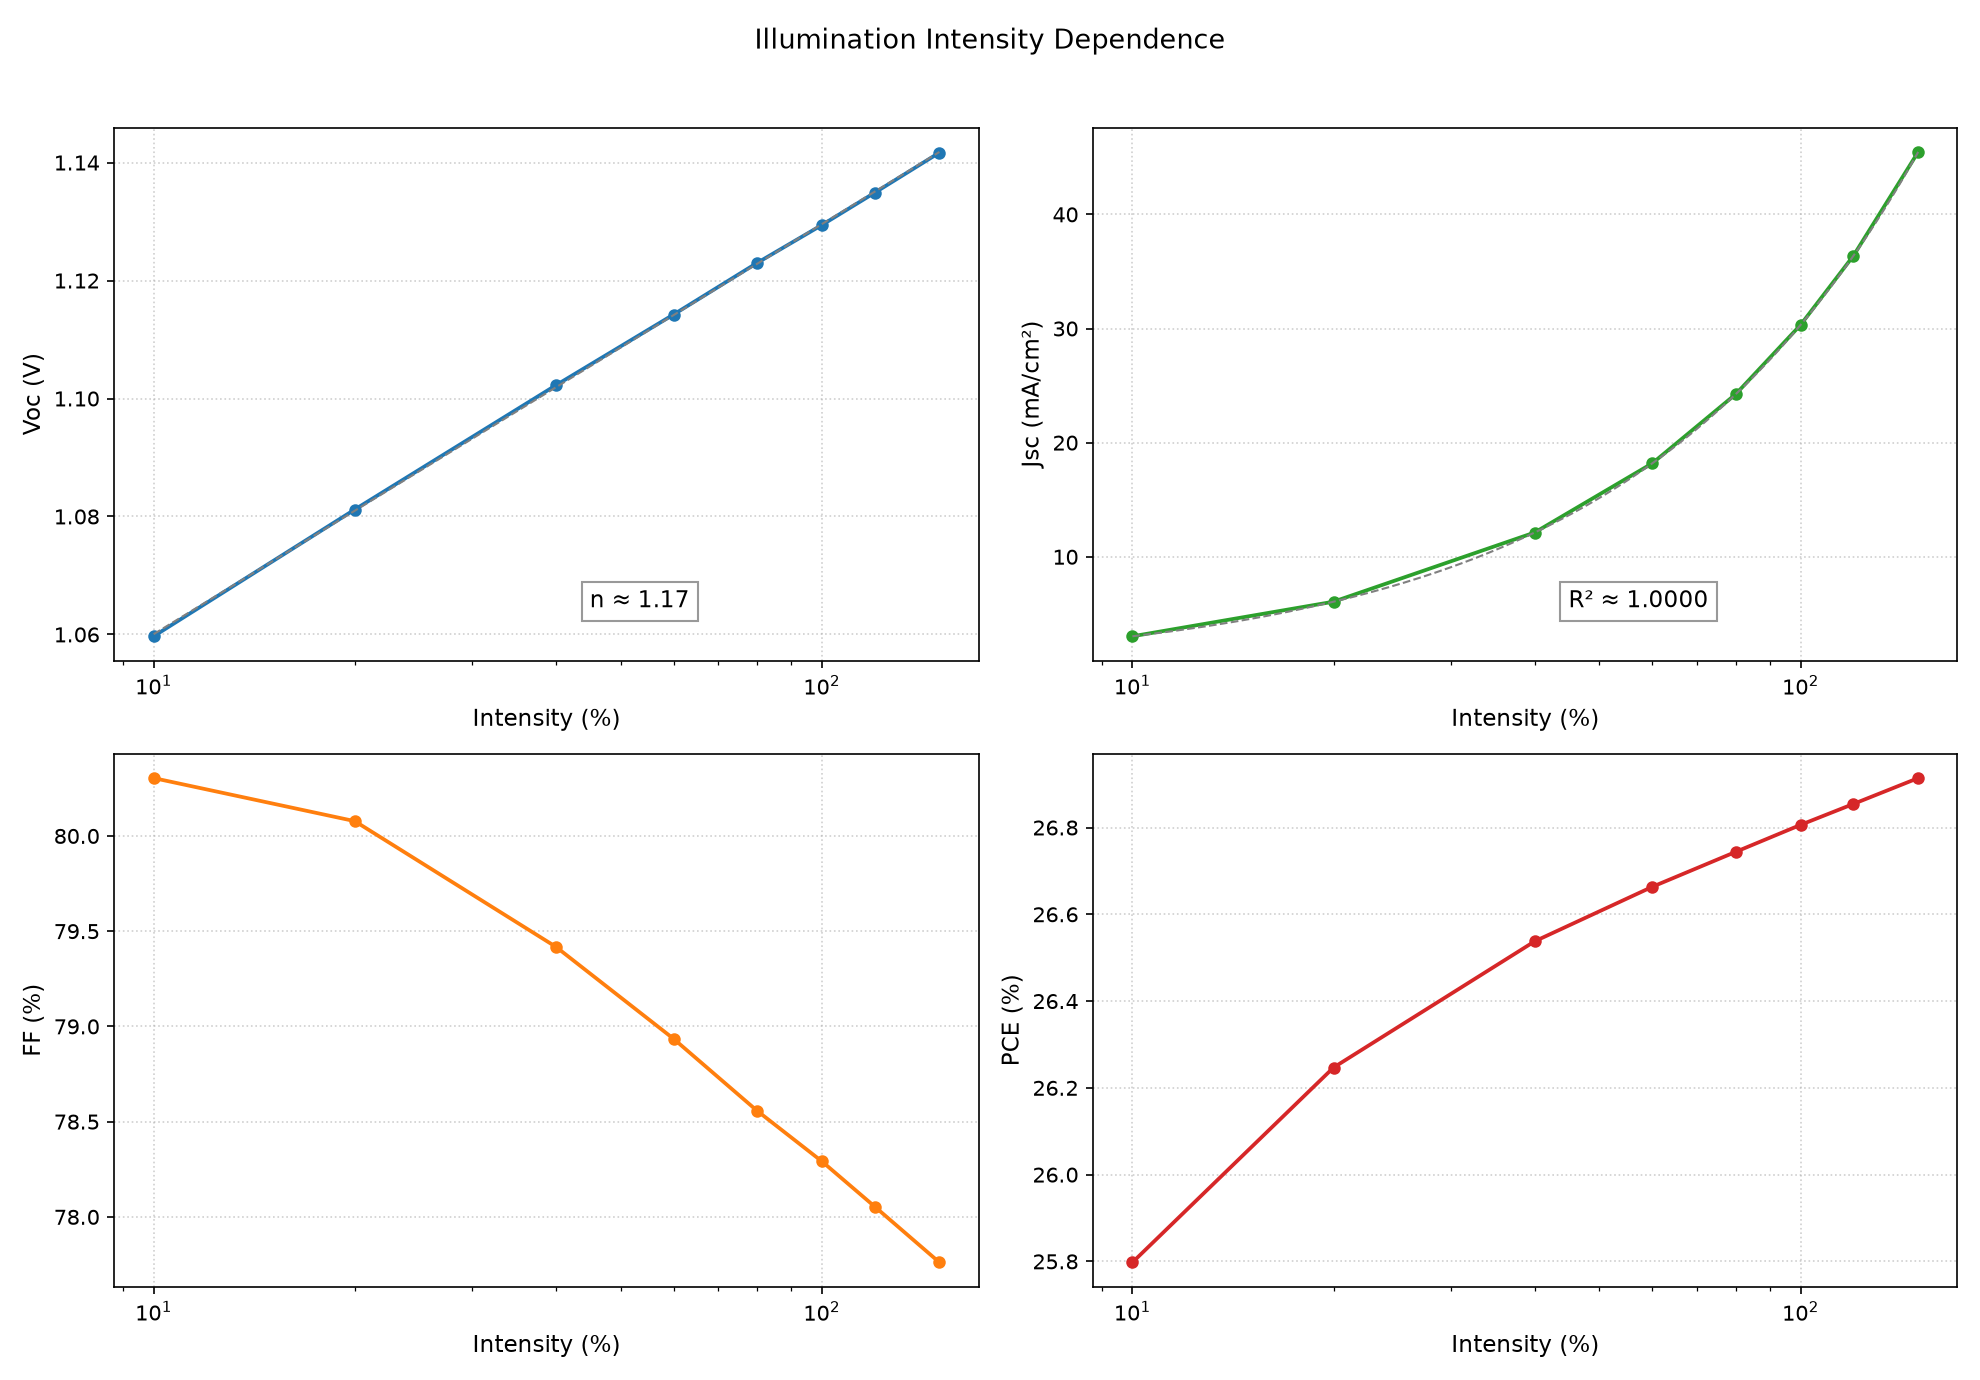
\includegraphics[width=0.85\linewidth]{figs/fig18.png}
\caption{Variation of photovoltaic parameters of the optimized device with illumination intensity from 0.1 to 1.5 suns.}
\end{figure}

\subsection*{Dark J--V characteristics}
Under dark bias (Figure S12) the cell rectifies hard: forward current at +1 V exceeds reverse current at $-$0.5 V by a factor of 1.8$\times$10$^{10}$, and leakage stays under 10$^{-10}$ A/cm$^{2}$ across the whole reverse window ($-$0.5 to +1.3 V). The exponential forward region fits to an ideality factor of n $\approx$ 1.5 and a reverse saturation current J0 $\approx$ 5$\times$10$^{-11}$ A/cm$^{2}$. Together these numbers describe high-quality bulk and interfaces with no measurable shunts.


\begin{figure}[htbp]
\centering
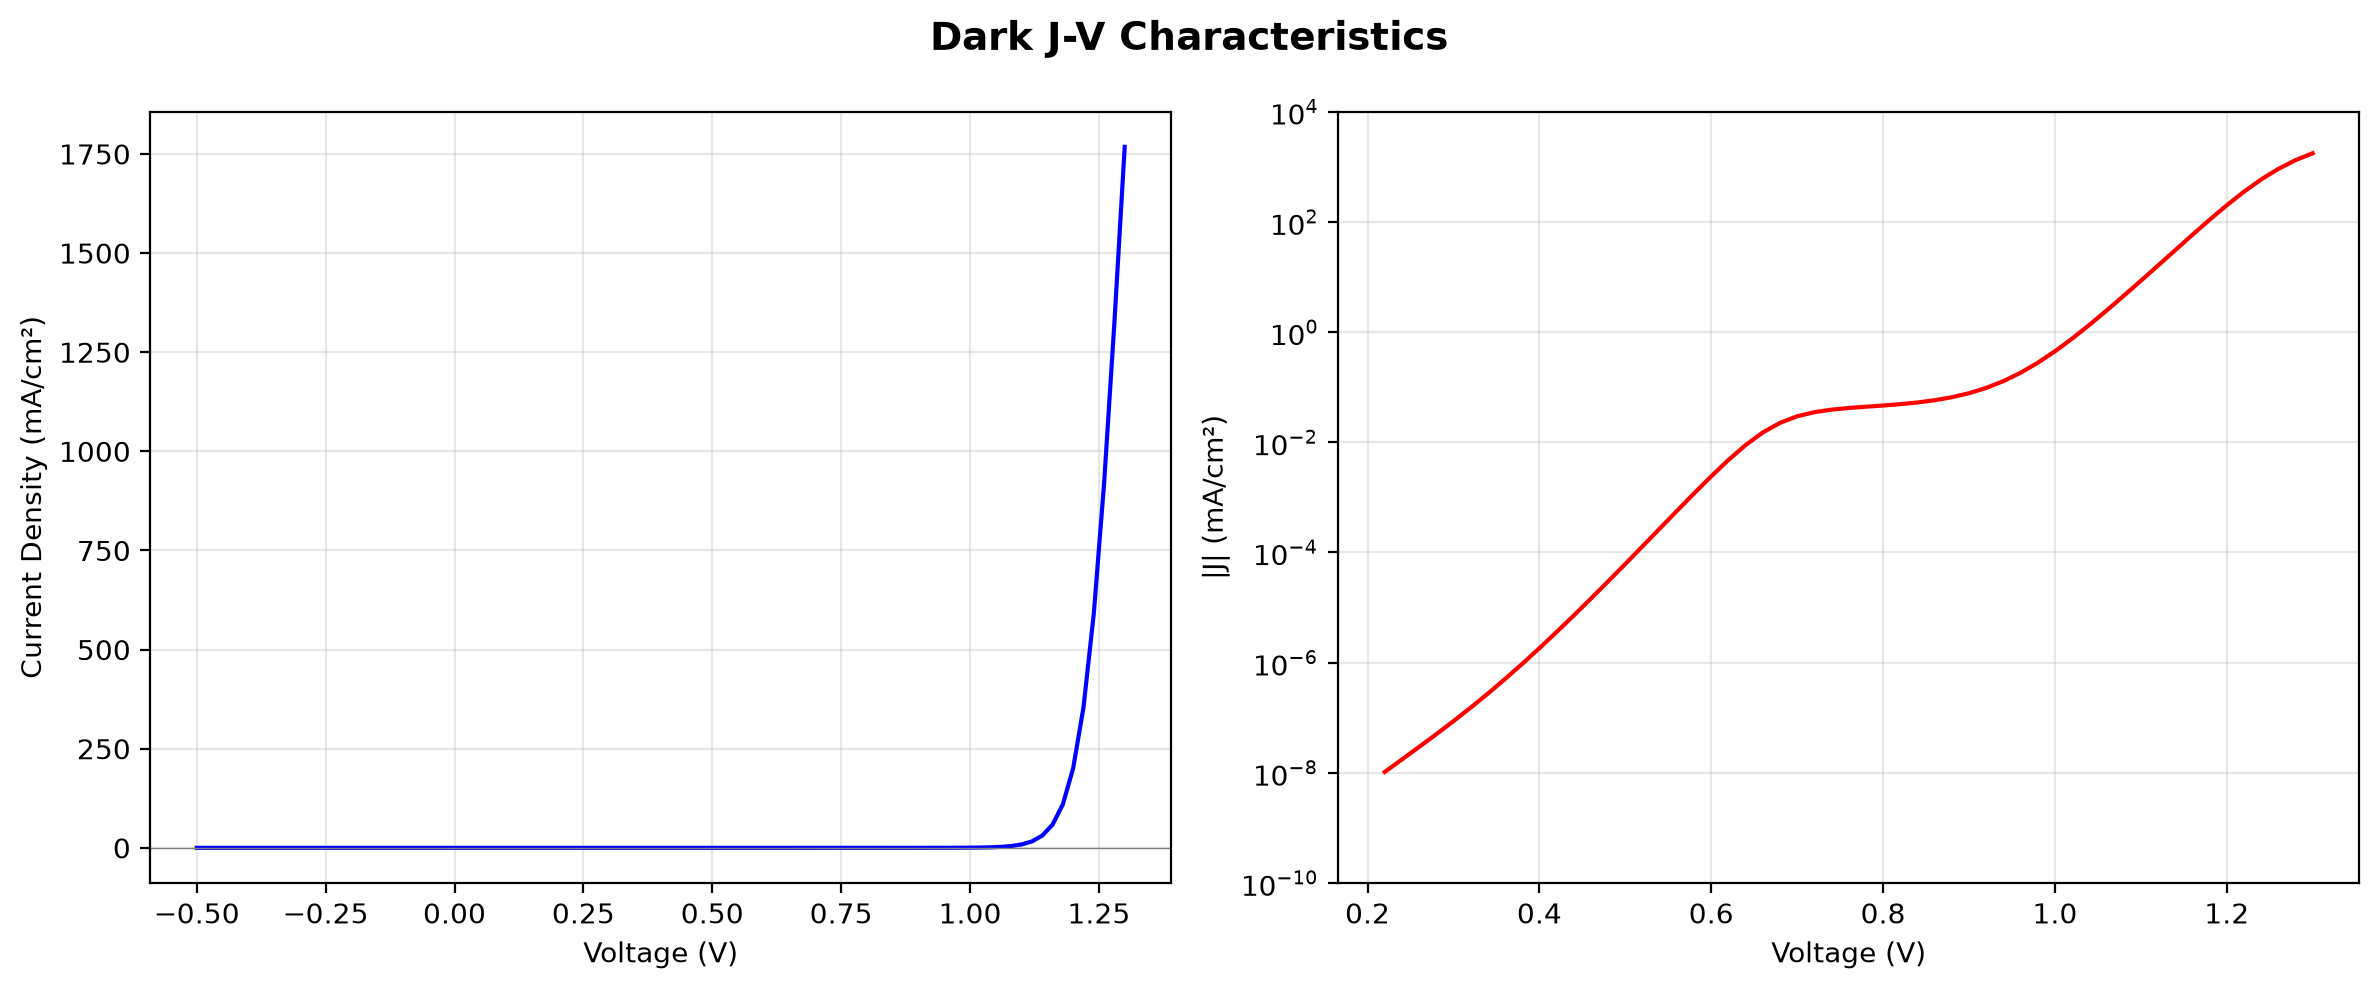
\includegraphics[width=0.85\linewidth]{figs/fig19.png}
\caption{Dark J--V characteristic of the optimized device. The forward branch is exponential over nearly three decades; the reverse branch remains below 10$^{-10}$ A/cm$^{2}$.}
\end{figure}

\begin{thebibliography}{99}
\bibitem{r35} W. Shockley and H. J. Queisser, ``Detailed balance limit of efficiency of p-n junction solar cells,'' J. Appl. Phys. 32(3), 510--519 (1961). doi:\url{10.1063/1.1736034.}
\bibitem{r36} S. Rühle, ``Tabulated values of the Shockley--Queisser limit for single junction solar cells,'' Sol. Energy 130, 139--147 (2016). doi:\url{10.1016/j.solener.2016.02.015.}
\bibitem{r37} C. H. Henry, ``Limiting efficiencies of ideal single and multiple energy gap terrestrial solar cells,'' J. Appl. Phys. 51(8), 4494--4500 (1980). doi:\url{10.1063/1.328272.}
\end{thebibliography}
\section*{S3.\ Screening and simulation setup tables}
\begin{table}[htbp]
\centering
{\small\setlength{\tabcolsep}{3pt}
\begin{tabularx}{\textwidth}{XXcX}
\hline
Study (Year) [Ref.] & Device Structure & PCE (\%) & Key Limitation
\\\hline
Pindolia et al. (2022) \cite{r14} & FTO/\allowbreak{}TiO$_{2}$/RbGeI$_{3}$/NiO/\allowbreak{}Ag & 9.77 & Broad multi-parameter sweep (HTL, ETL, thickness, doping, defects, back contact, temperature); baseline efficiency remains modest and Ge$^{2+}$ oxidation not addressed.\\
Saikia et al. (2022) \cite{r24} & FTO/\allowbreak{}TiO$_{2}$/CsGeI$_{3}$/CuI/\allowbreak{}Au & 10.80 & No multi-HTL comparative analysis.\\
Bouazizi et al. (2022) \cite{r15} & FTO/\allowbreak{}PCBM/\allowbreak{}CsSn0.5Ge0.5I3/\allowbreak{}Spiro/Au & 18.13 & Mixed Ge/Sn absorber; thermal sensitivity.\\
Loumachi et al. (2024) \cite{r22} & ITO/\allowbreak{}C$_{60}$/RbGeI$_{3}$/CBTS/\allowbreak{}Ag & 27.21 & Optimized RbGeI$_{3}$ thickness and series/shunt resistance; interface defect optimization not addressed.\\
Raj et al. (2025) \cite{r39} & FTO/\allowbreak{}TiO$_{2}$/RbGeI$_{3}$/PEDOT:PSS/\allowbreak{}Au & 18.60 & Organic HTL limits long-term stability.\\
Pathak et al. (2026) \cite{r23} & FTO/\allowbreak{}TiO$_{2}$/RbGeI$_{3}$/Spiro-OMeTAD/\allowbreak{}Au & 26.47 & Ge$^{2+}$ $\rightarrow$ Ge$^{4+}$ oxidation not addressed; only single ETL/HTL combination studied.\\
Dash et al. (2025) \cite{r17} & DFT + SCAPS-1D of RbGeX$_{3}$ (X=Cl, Br, I) & 25.76 & Primarily material-level comparison; limited device-architecture optimization.\\
\hline
\end{tabularx}
}
\caption{Table S1. Summary of recent SCAPS-1D studies on lead-free Ge-based and Sn-based perovskite solar cells.}
\end{table}
\begin{table}[htbp]
\centering
{\footnotesize\setlength{\tabcolsep}{3pt}
\begin{tabularx}{\textwidth}{Xcccc}
\hline
Parameter & TiO$_{2}$ & FTO & RbGeI$_{3}$ & CuI
\\\hline
Thickness (nm) & 30 & 500 & 400 & 100\\
Bandgap $E_{\mathrm{g}}$ (eV) & 3.2 & 3.2 & 1.4 & 3.1\\
Electron affinity $\chi$ (eV) & 4.0 & 4.4 & 3.9 & 2.1\\
Dielectric permittivity $\epsilon$r & 9 & 9 & 23.01 & 6.5\\
CB effective DOS N$_{\mathrm{C}}$ (cm$^{-3}$) & 2$\times$10$^{18}$ & 2.2$\times$10$^{18}$ & 1.4$\times$10$^{19}$ & 2.8$\times$10$^{19}$\\
VB effective DOS N$_{\mathrm{V}}$ (cm$^{-3}$) & 1.8$\times$10$^{19}$ & 1.8$\times$10$^{19}$ & 2.8$\times$10$^{19}$ & 1$\times$10$^{19}$\\
Electron mobility $\mu$e (cm$^{2}$ V$^{-1}$ s$^{-1}$) & 20 & 20 & 28.6 & 100\\
Hole mobility $\mu$p (cm$^{2}$ V$^{-1}$ s$^{-1}$) & 10 & 10 & 27.3 & 43.9\\
Donor density $N_{\mathrm{D}}$ (cm$^{-3}$) & 9$\times$10$^{16}$ & 1$\times$10$^{19}$ & 1$\times$10$^{9}$ & 0\\
Acceptor density $N_{\mathrm{A}}$ (cm$^{-3}$) & 0 & 0 & 1$\times$10$^{9}$ & 1$\times$10$^{18}$\\
Bulk defect density $N_{\mathrm{t}}$ (cm$^{-3}$) & 1$\times$10$^{15}$ & 1$\times$10$^{14}$ & 1$\times$10$^{15}$ & 1$\times$10$^{15}$\\
\hline
\end{tabularx}
}
\caption{Table S2. Initial electrical and optical parameters used in the SCAPS-1D simulation of the proposed FTO/\allowbreak{}TiO$_{2}$/RbGeI$_{3}$/CuI/\allowbreak{}Au solar cell.}
\end{table}
\begin{table}[htbp]
\centering
{\small\setlength{\tabcolsep}{3pt}
\begin{tabularx}{\textwidth}{Xc}
\hline
Interface & Interface defect density $N_{\mathrm{t}}$ (cm$^{-2}$)
\\\hline
TiO$_{2}$ / RbGeI$_{3}$ & 1 $\times$ 10$^{14}$\\
RbGeI$_{3}$ / CuI & 1 $\times$ 10$^{14}$\\
\hline
\end{tabularx}
}
\caption{Table S3. Initial interface defect density applied at each heterojunction.}
\end{table}
\begin{table}[htbp]
\centering
{\small\setlength{\tabcolsep}{3pt}
\begin{tabularx}{\textwidth}{XX}
\hline
Parameter & Value
\\\hline
Simulation software & SCAPS-1D version 3.3.10\\
Illumination spectrum & AM 1.5G\\
Incident power density & 100 mW/cm$^{2}$ (1000 W/m$^{2}$)\\
Operating temperature & 300 K (27 $^{\circ}$C)\\
Illumination intensity & 1 Sun\\
Scan mode & Illuminated J--V\\
Device type & Planar heterojunction\\
Front contact & FTO\\
Back contact & Au\\
Initial material parameters & Table II\\
Initial interface defect density & Table III\\
\hline
\end{tabularx}
}
\caption{Table S4. Simulation conditions used in SCAPS-1D.}
\end{table}
\end{document}